\documentclass{article}
\usepackage{naturetex}
%如果要中文,写:
\usepackage{ctex}
\usepackage{multicol} %用于实现在同一页中实现不同的分栏
\renewcommand{\baselinestretch}{1.5}
\usepackage{graphics}
%\usepackage{graphicx}
\usepackage{amsmath}
\usepackage{hyperref}
%\usepackage{subcaption}
\usepackage{subfigure}
\usepackage{multirow}
\hypersetup{
	colorlinks=true,
	linkcolor=black
}
%\usepackage{subfig}
\usepackage{float}
\begin{document}

% Keywords command
\providecommand{\keywords}[1]
{
	\small	
	\textbf{\textit{关键词:}} #1
}
\maketitle

{\setstretch{1.0}
	% *** ABSTRACT ***
\begin{abstract}
	爱彼迎是一家共享民宿在线短租平台,随着共享理念在国内的兴起,中国越来越多的房东通过爱彼迎出租自家民宿。面对新兴市场,怎样为房源定价才能使房东获得最多收入成为爱彼迎平台和房东共同关心的问题。本文从需求和价格之间关系的角度出发,利用弹性网络、支持向量回归、LightGBM和多层感知机预测北京市爱彼迎房源的预订率。并选取典型房东,预测其不同定价下的预定率从而计算预期收入,进而向房东提出定价建议。
	\par 本文主要创新点在于不同于以往直接预测共享民宿的价格,而是使用机器学习的方法预测需求进而提出定价建议;并填补了中国共享民宿行业中房东定价问题的空白。
\end{abstract}
\keywords{共享民俗,机器学习,需求预测,定价管理}
}% setstretch
\newpage
\tableofcontents
% *** INTRO ***
\newpage
\begin{multicols}{2}
\section{说明}
这一版本和上一版本之间主要有如下改变:
\begin{enumerate}
	\item 更新了数据。将数据从去年十二月更新到了今年六月
	\item 更新了排版。图片更新为dpi=300的质量,并调整了大小,尽量使其更加合乎要求。
	\item 更新了部分结论。
\end{enumerate}
\section{介绍}
2010年在线短租行业在国内兴起,具有广阔的发展前景。其运营模式主要是通过互联网构建一个双边市场交易平台,将房东和房客都集中到这一平台中,通过降低信息不对称和搜寻成本的不利影响,提高房与房客的匹配效率,而提供交易平台的企业则从中获取一定数额的中介费用。这种模式鼓励有效利用空余房源,降低空置成本,使房屋多样化得到增值,对传统住宿消费市场而言,有两方面优势:一、相比于酒店预订房源覆盖广,种类多、选择丰富,消费灵活;性价比高,同等价位下,享受酒店所不具备的个性体验;二、相比于传统线下短租——在线短租网站/平台房源的丰富性,为租客提供多种选择;展示信息形式多样,提高沟通效率,降低交易双方的信息不对称性;平台的保障机制,能有效降低预订和支付环节可能的交易风险。
\par 爱彼迎(Airbnb)成立于2008年8月,总部设在美国加州旧金山市,作为在线短租平台的主要参与者,用户可通过他的网络或手机应用程序发布、搜索度假房屋租赁信息并完成在线预订。2015年6月底,Airbnb完成了15亿美元的融资,估值达到310亿美元,成为仅次于Uber、小米的全球估值第三高的科技创业公司,同年8月,正式进军中国内地。\cite{中国在线短租行业发展报告}
\par 在中国的运营中,爱彼迎主要通过向房东收取10\%提成的方式赚取收益,这种运营模式将爱彼迎的收入与房东的收入挂钩,房东收入越高,爱彼迎平台收入才能更高,据统计,大部分房东主要是通过在爱彼迎上发布房间来赚取利润。因此怎样定价能使得房东能够得到最大收益自然也就成了爱彼迎和房东共同关心的问题。
\par 本文主要通过机器学习的方法预测爱彼迎平台上房源的房客预订率。结合经济学价格需求曲线的理论尝试寻找房价定价不合理的典型房东,通过机器学习模型,预测该房东在不同的定价下的预订率,给出该房东的价格制定区间的建议。
\par 本文其余章节的主要思路如下:
\begin{enumerate}
	\item 在相关研究一章中讨论定价管理方面的相关研究,指出这些研究的不足之处并详细阐明本文研究的不同之处。
	\item 在数据处理及探索性分析一章中,描述了数据来源、对重点特征的单变量探索性分析、多个数据之间的相关性分析,并说明了数据的清洗、处理过程。
	\item 在方法一章中描述本文主要用到的方法,包括弹性网络、支持向量回归、LightGBM、多层感知机几种典型的方法,介绍参数寻优的方法以及参数寻优的结果。
	\item 在结果一章中评价模型的表现,给出最重要的特征,并根据结果提出建议。
	\item 在典型房东分析一章中,尝试利用学习得到的最优模型进行处理,分析典型的房东,同时展示出这个模型的优点和不足。
\end{enumerate}
\section{相关研究}
本文从现有数据出发研究房东怎样定价,研究的范围包括爱彼迎中国在北京的所有共享民宿房东。定价方面有很多相关管理学理论或模型作为指导,不同的领域发展出了不同的理论,包括定价需求模型、定价的博弈论模型等\cite{ozer2012oxford},这些不同的理论大都来自理想化的假设(如理性经济人假设、边际效用理论)等以及公式推导,只有利用数据的支持才能展现出效果。
\par 在数据驱动的相关研究方面,主要包括使用计量方法和机器学习预测方法两种主要思路。Wang 和 Nicolau\cite{wang2017price} 研究了共享经济的价格决定因素,通过使用最小二乘和分位数回归分析方法分析 Airbnb 房源价格。在一项类似的研究中,Masiero等人\cite{masiero2015demand} 使用分位数回归模型分析出行的特征和度假屋以及酒店价格之间的关系。在一项更简单的工作中,Yang 等人\cite{yang2016market} 应用线性回归研究市场可及性之间的关系和加勒比地区的酒店价格,其中他们认为用户评分和酒店等级是重要的影响因素。Neloy等利用公寓信息和价格的数据以及集成学习模型进行的房租价格预测\cite{文献综述-房屋价格预测},李等人\cite{li2016reasonable}还使用了一种聚类+线性回归的方法创建不同城市的Airbnb房源价格预测模型,他们将物业与城市的距离地标作为聚类特征。Kalehbasti等人\cite{kalehbasti2019airbnb}利用纽约市数据进行预测,希望以此作为指导房东定价的依据。
\par 上述研究中,在面对爱彼迎的房源数据时都有不完善之处。计量的方法试图通过寻找和分析关键指标,确定影响房价或需求的关键因素,但是这些应用面临的场景主要是OTA领域,即面对一个标准化的房源,通过衡量房源的位置、规格等,即可给出房源的定价一个较为合理的估计,这些应用在多样化的共享平台的房源暂时还没有得到良好的表现。而关于机器学习的方法,主要集中在通过一系列因素预测房源价格上,而爱彼迎房源价格直接进行预测并不合理:首先,爱彼迎平台房源价格的并非完全按照客观规律进行制定,规定爱彼迎房源价格的只有房东,房客只有选择住与不住的权力,这种定价属于“挂牌价”的定价策略\cite{ozer2012oxford},这种定价策略和股市交易、石油价格等能在很快时间内达到市场均衡的定价方式是不一样的,房东目前的定价并不满足市场均衡的前提;另外,爱彼迎房源的房东大多是兼职,这和普通的酒店供应者等的情况不同,房东并没有足够的时间精力以及财力去收集足够的短租市场的信息,也就不能保证掌握足够的技巧制定合适的价格。因此,如果使用这种机器学习方法预测爱彼迎平台的房源价格,即使学习出不错的模型模拟房东定价,也对于新进入的房东没有足够的借鉴意义。
\par 基于上述分析,本文尝试利用机器学习模型研究房源的定价管理,在前人的基础上吸收计量方法的优点。主要贡献如下:模型并不直接预测价格,而是从需求的角度进行预测。把预订率作为需求的指标,首先尝试学习出爱彼迎房源的特征与预订率的关系,之后挑选表现最好的模型验证价格和预订率之间的关系,接着利用学习出来的模型尝试给出定价建议。这种研究模式尽量避免了前文所述的面对多样化、房东定价本身并不合理的两个问题。
\section{数据处理及探索性分析}
北京市的公共 Airbnb 数据集被用作主要数据本研究的数据来源。\cite{data-insideairbnb}该数据集是截至2021年10月26日所有北京市爱彼迎在线房源数据,主要使用了该数据集中的3张csv表格,通过合并这些表格,获得了包含每个房源的地理位置、所在行政单位、评价、价格、上线时间、未来365天可预订数等信息的数据框。最终用来机器学习的数据框包含19675个样本,每个样本有116个特征。图\ref{图:房价数据}显示了该数据集中挂牌价格和预订率的地理分布,图中可以看出房源大多集中在北京的中西部地区,且房价、预订率和地理位置之间没有十分显著的关系。
\begin{figure*}
	\centering
	\subfigure[位置和房价关系。价格取值从0到30000左右,但大部分房价在5000以下]{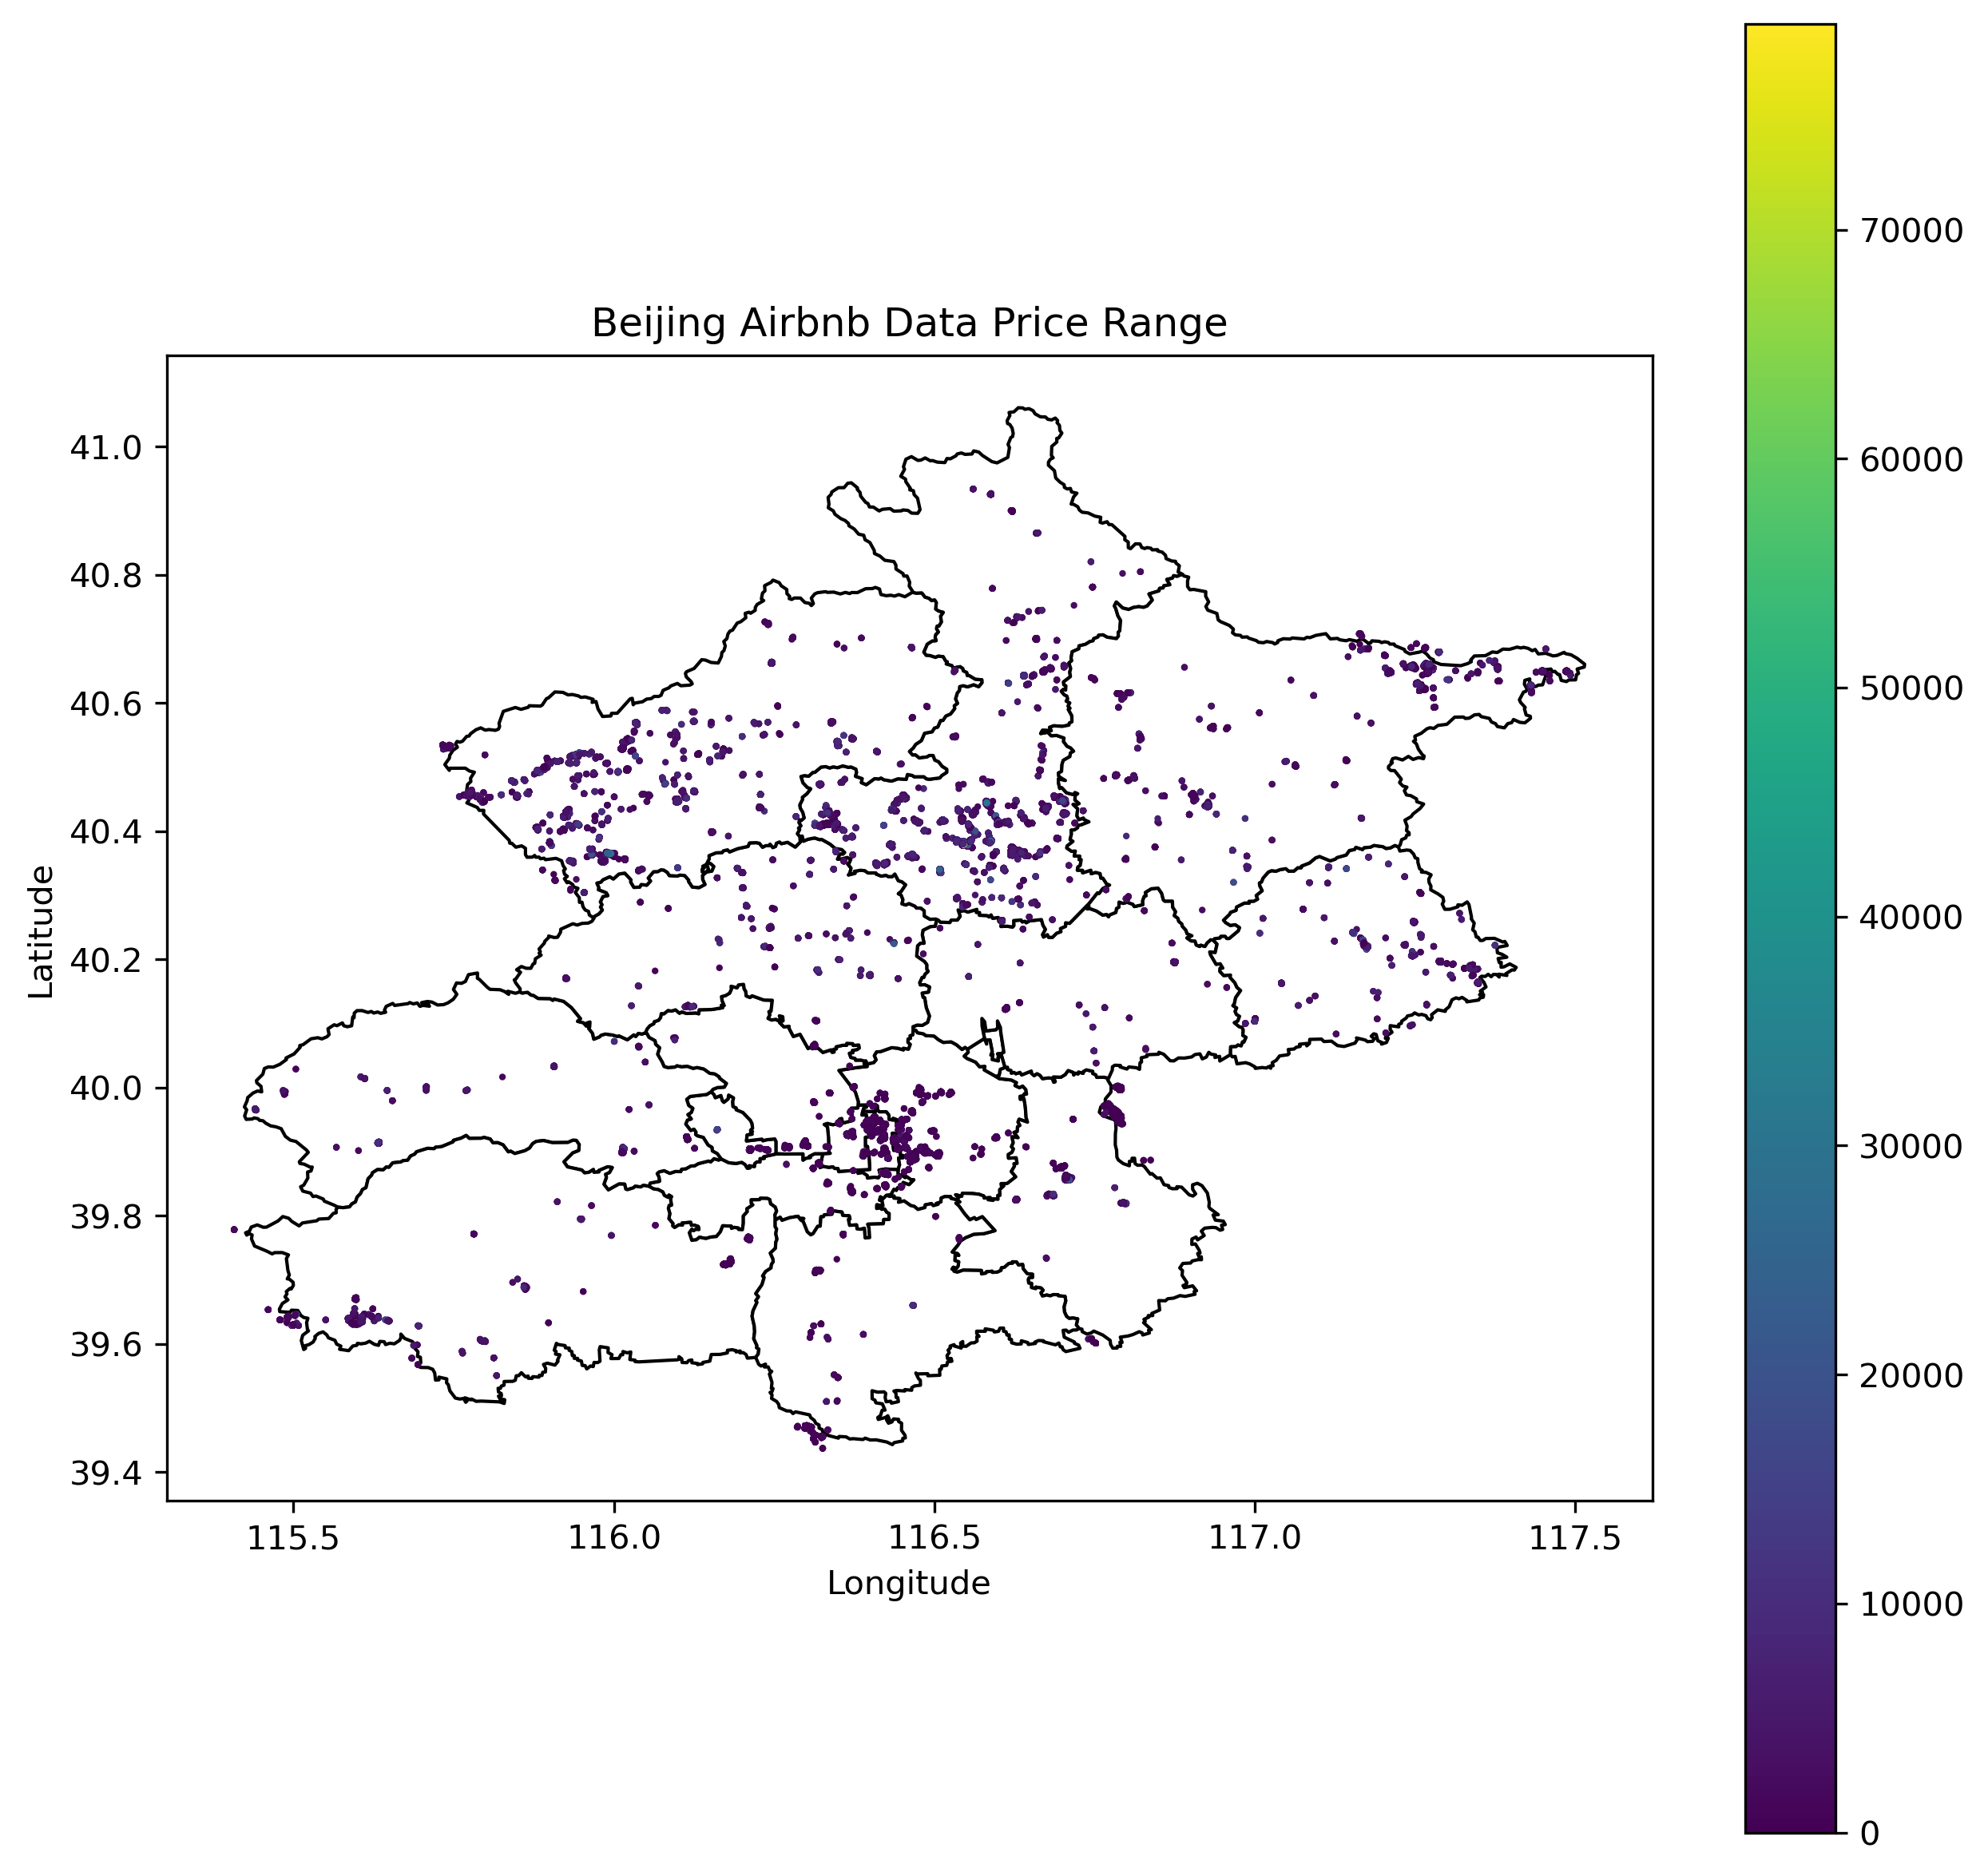
\includegraphics[width=0.45\linewidth]{地理-房价}} 
	\subfigure[位置和预订率关系。从图中可以看出,位置和预订率之间没有显著关系。]{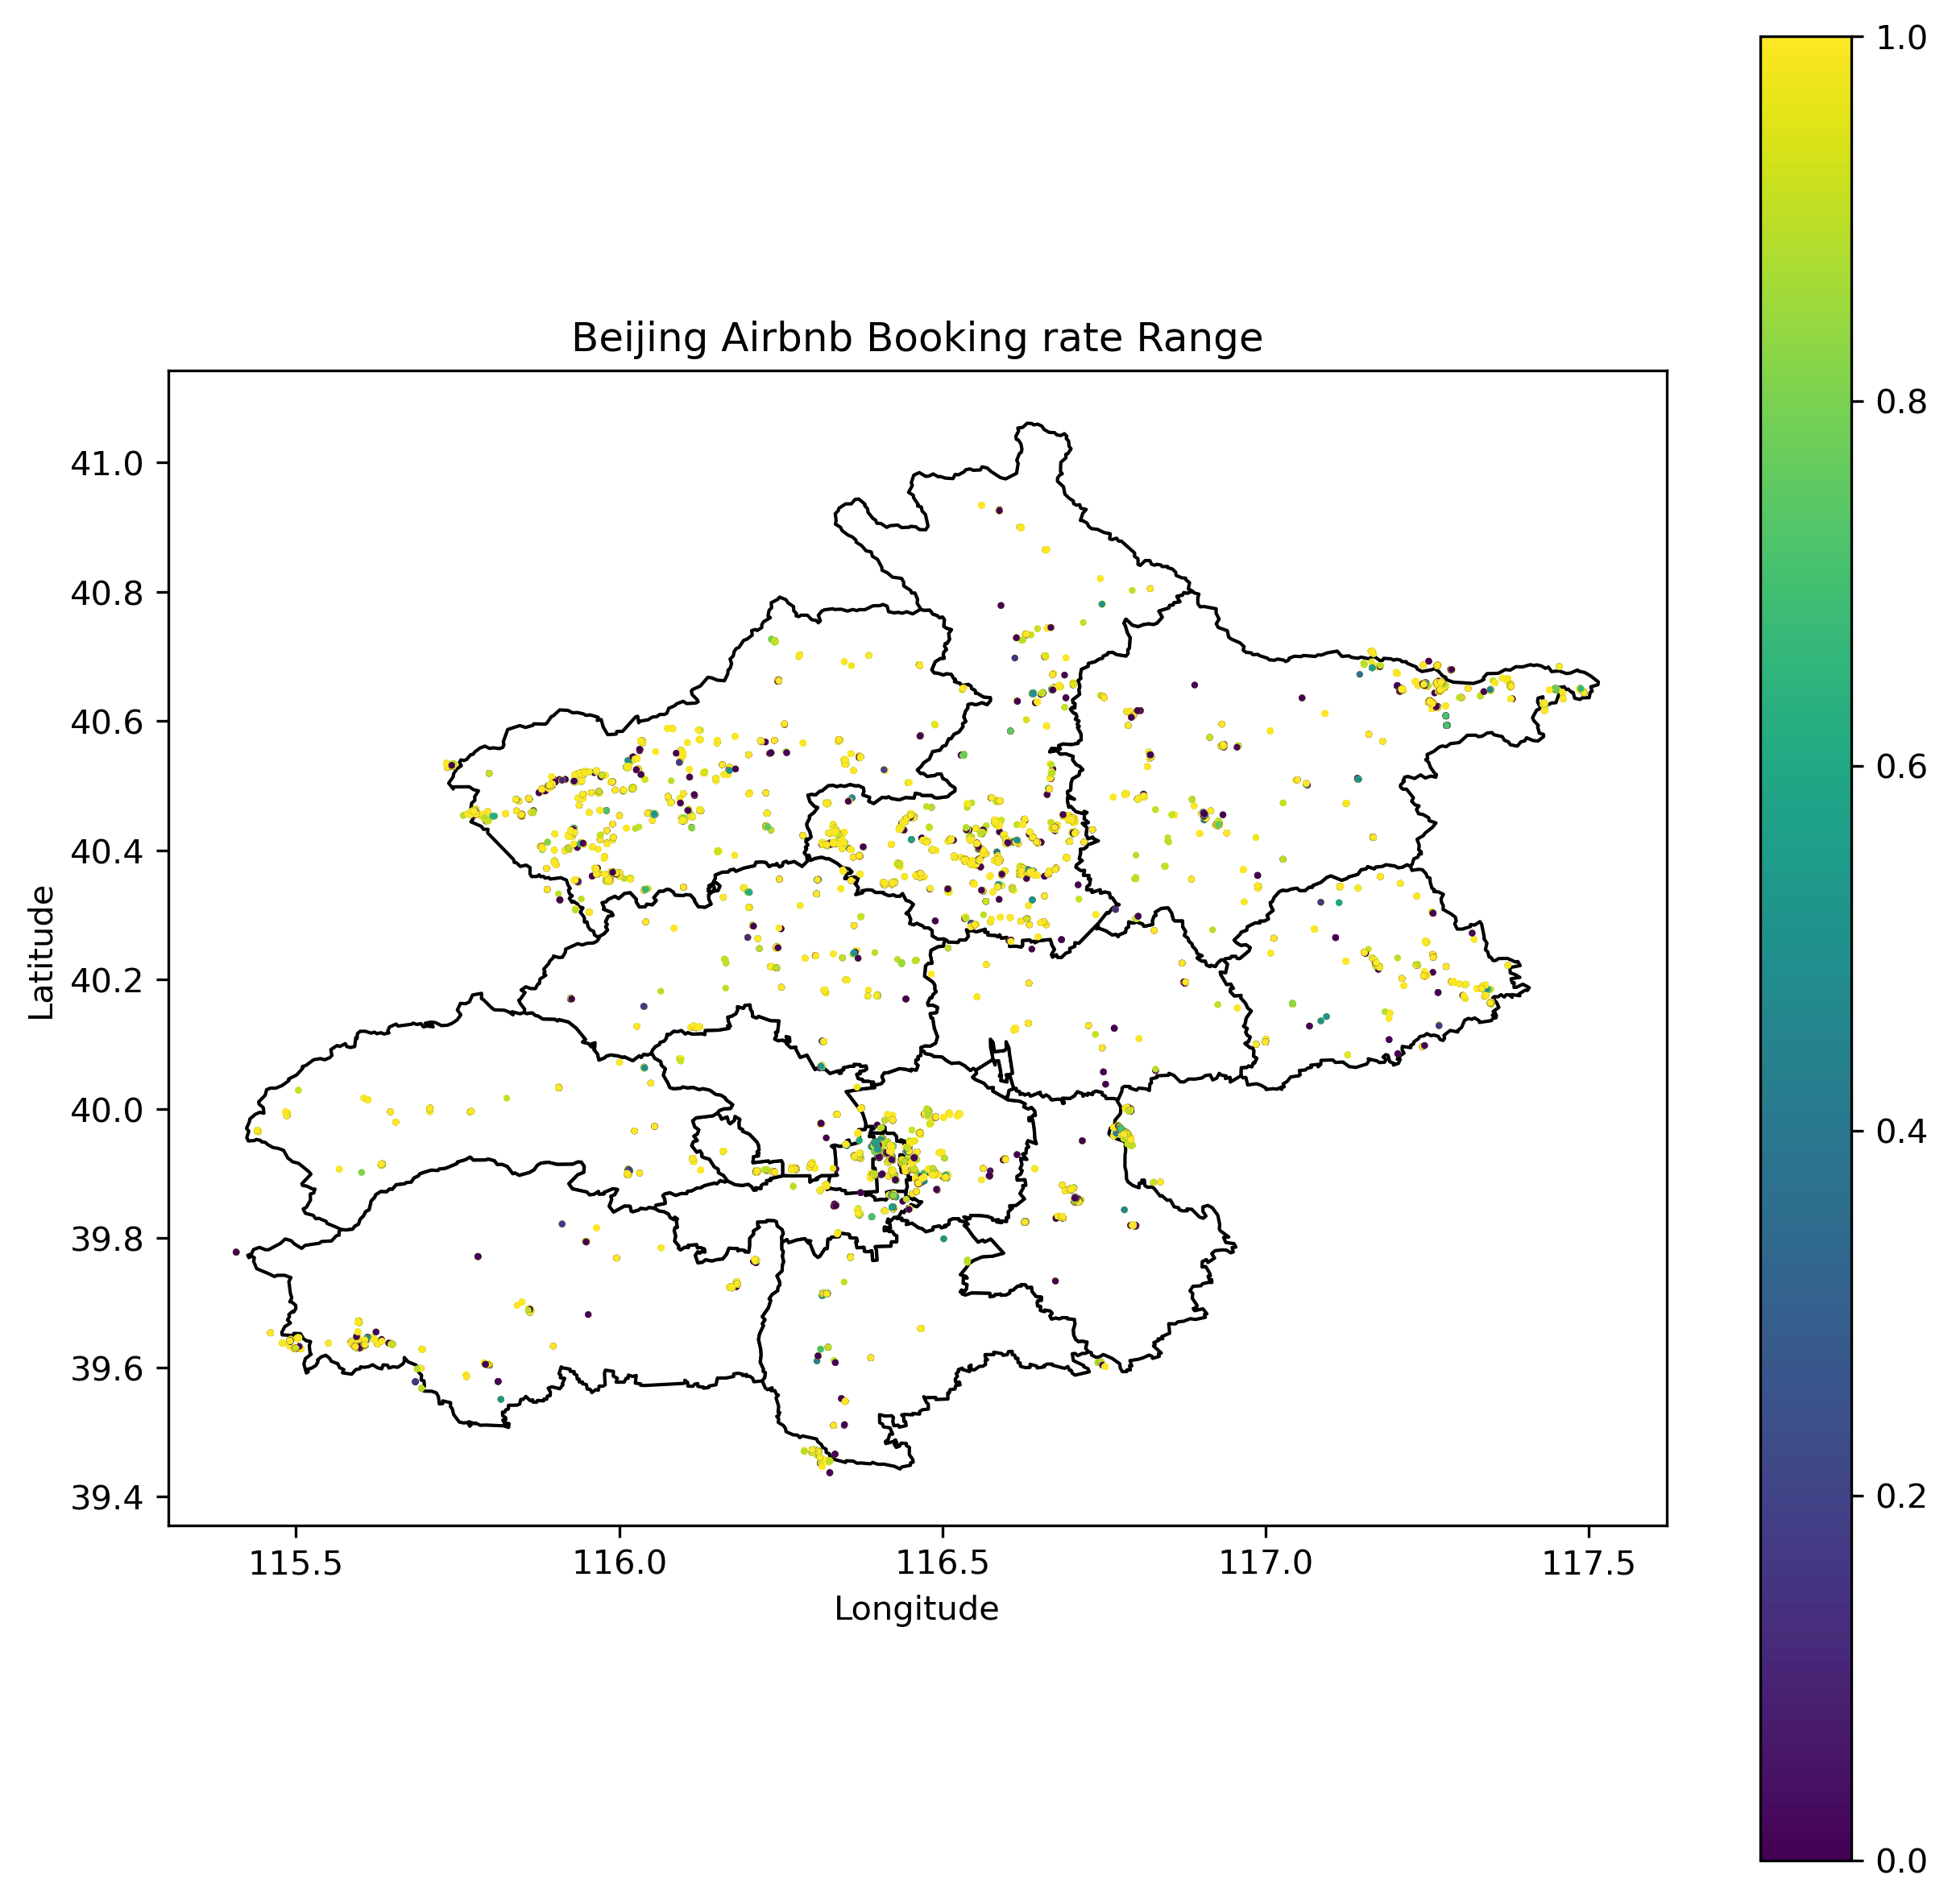
\includegraphics[width=0.4\linewidth]{地理-预订率}}
	\caption{地理信息}
	\label{图:房价数据}
\end{figure*}
具体而言,主要使用到的处理方法如下:
\begin{enumerate}
	\item 删除具有频繁且不可修复的缺失字段的特征或在适当的情况下将缺失值设为0。
	\item 将一些特征转换为浮点数(例如,通过删除价格中的美元符号)。
	\item 删除不相关或无信息的特征,如主页网址。
	\item 使用情感分析的方法进行特征评论信息。
	\item 将所有数据进行归一化处理。
\end{enumerate}
\par 在数据划分方面,主要利用sklearn进行自动划分,数据分为三组;即,训练集(包括75\%的原始数据)和测试集(占 25\%原始数据),验证集通过训练集的5折交叉验证实现。
\subsection{评论数据情感分析}
考虑到类似研究认为客户评论对于房源的出租率具有重要影响\cite{Petz2013Jul},为了提高预测模型的准确性,对房源能够记录到的所有评论利用SnowNLP\cite{snownlp}和Textblob\cite{Ttestblob}两个包分别计算评论数据的情绪值,按照加权赋分的方法将两个包计算得到的情感值进行合并,对每个房源的所有评论数据计算平均总情感,完成提取评论信息的过程。利用更加细致的方法分析客户情感也是未来可能的改进方向。\cite{Petz2013Jul}。
\par 每个情感数据分析结果如图\ref{图:情感分布},从图中可以看出平均情感值大都在-1到1之间,属于无偏分布。
\begin{figure}[H]
	\centering
	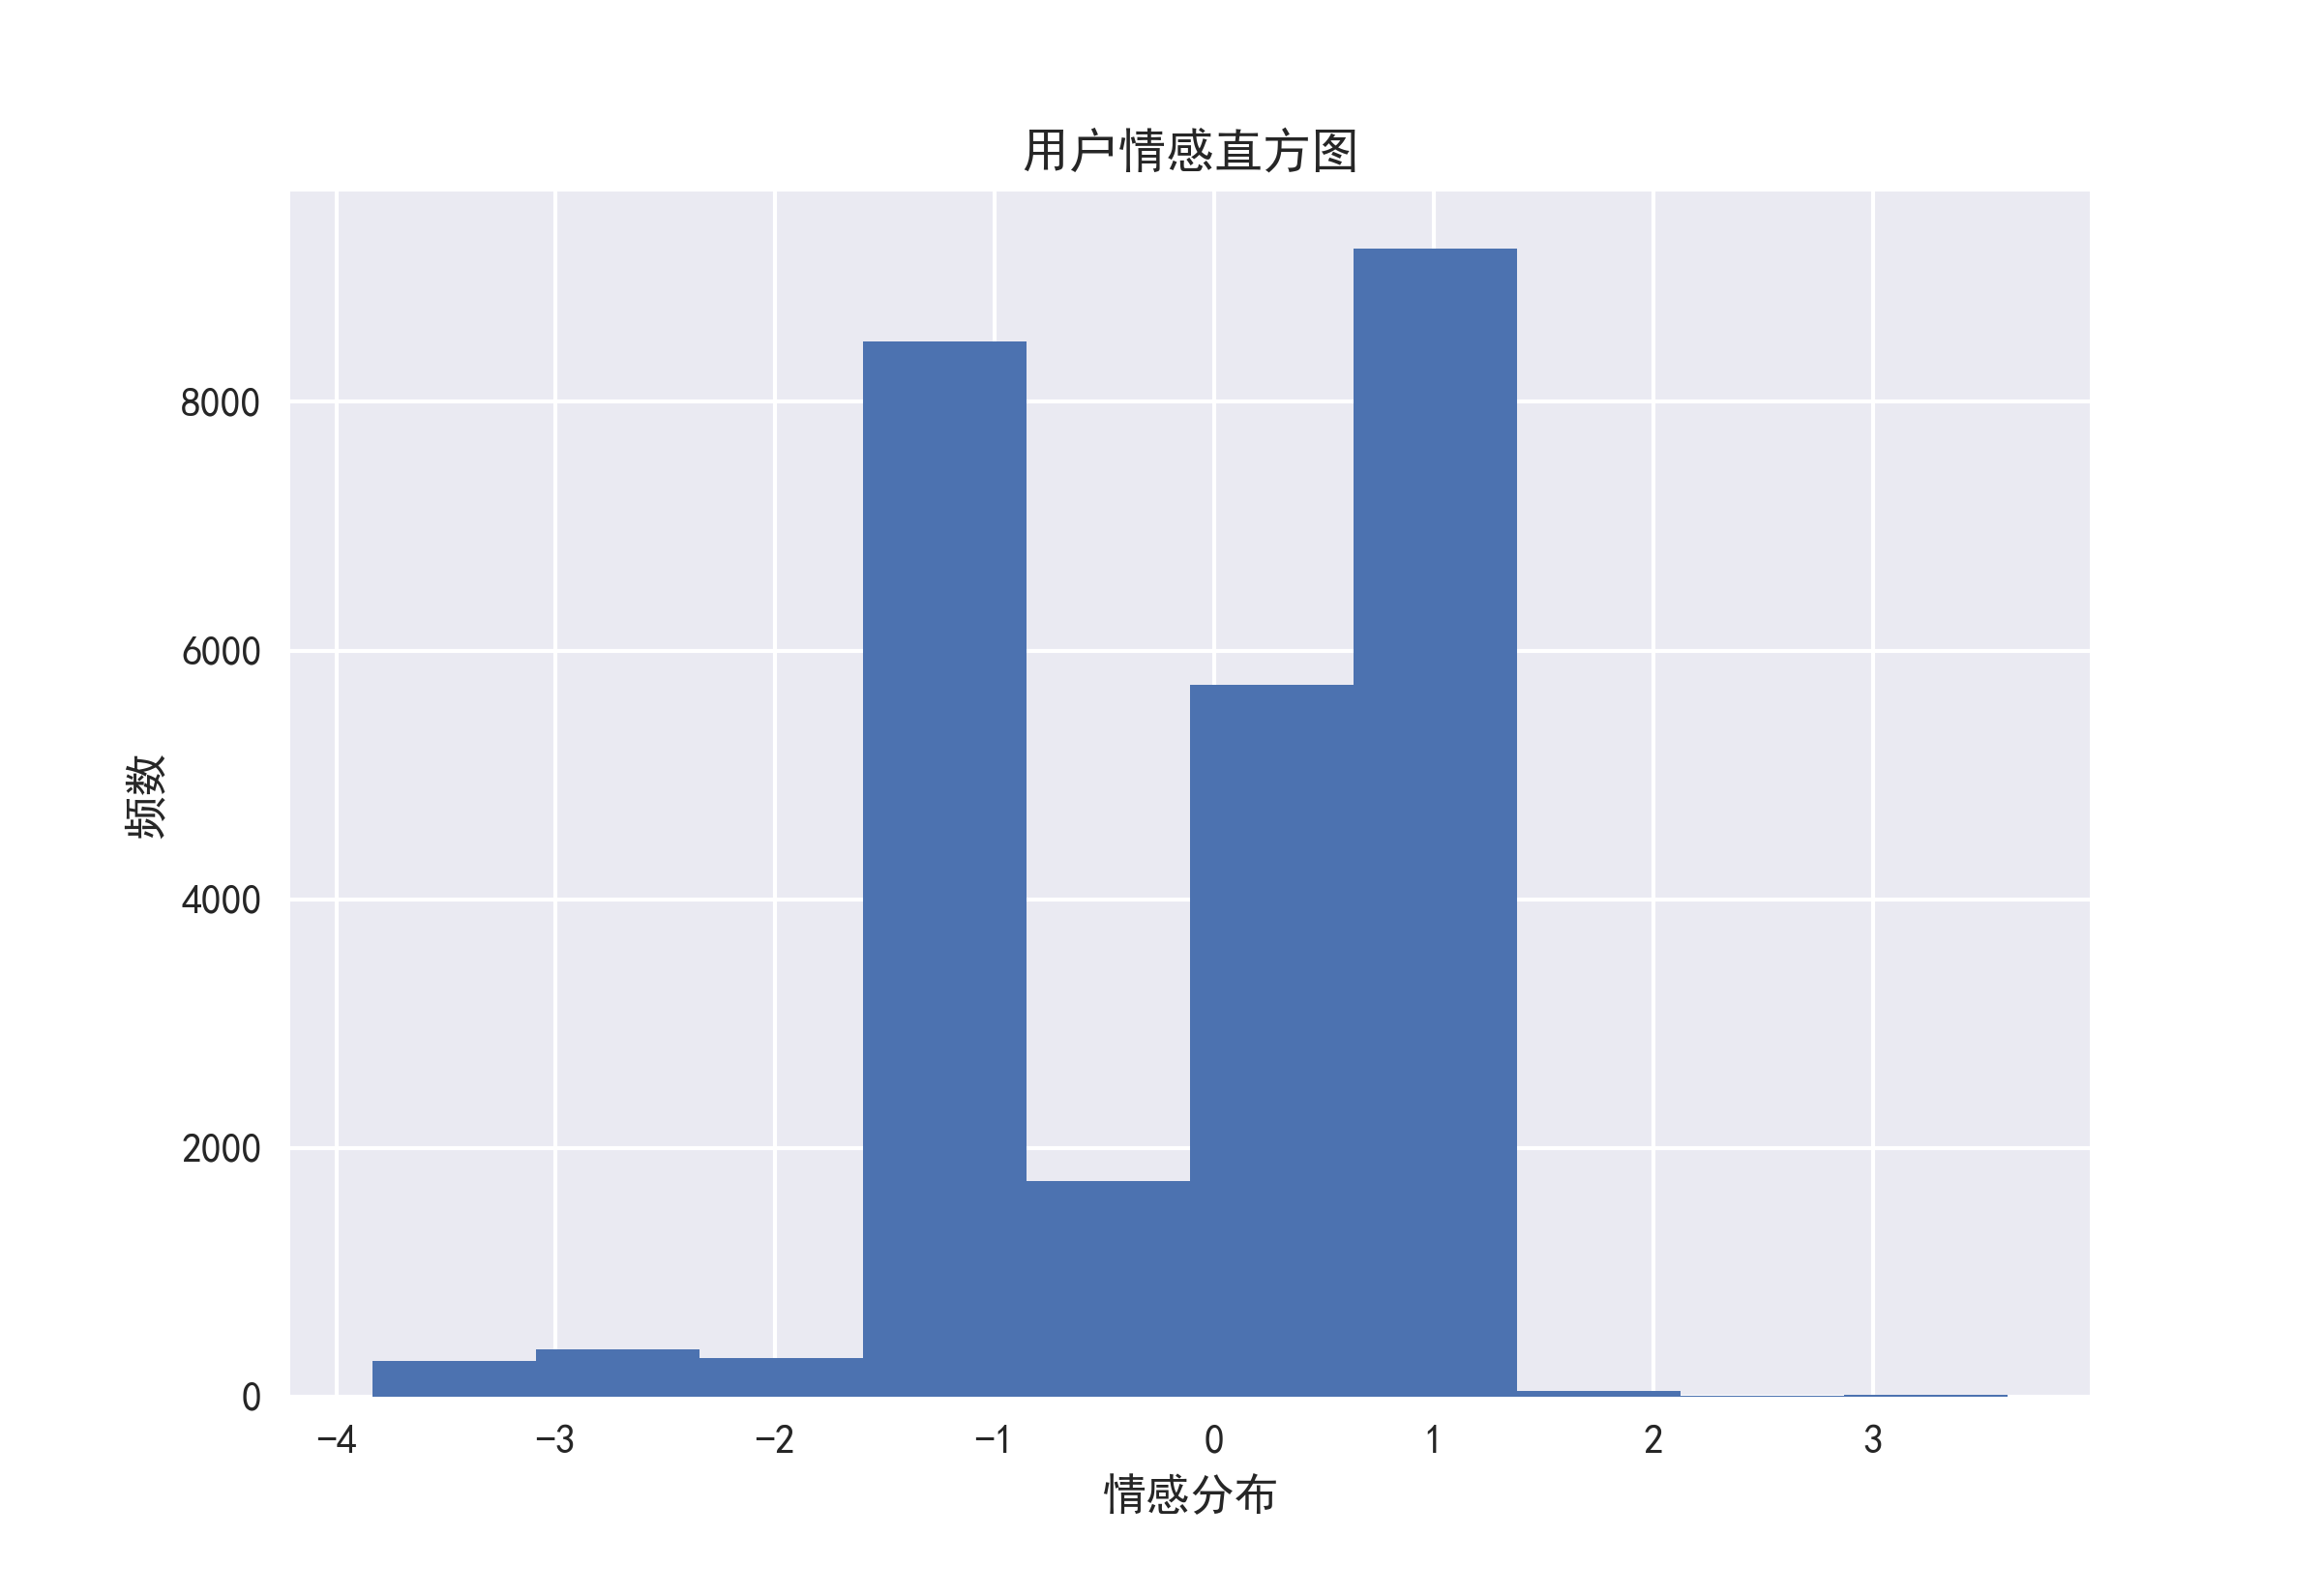
\includegraphics[width=0.8\linewidth]{情感分布直方图}
	\label{图:情感分布}
	\caption{评论情感分布图。图中x轴代表了标准化之后的情感数据,y轴代表出现的频数,图中展现出较为近似的正态分布。}
\end{figure}
\subsection{价格探索性分析}
价格也是影响需求(房源预订率)的重要指标,需要展开进行分析。如图\ref{fig:价格分布},价格呈现明显的偏态分布,鉴于价格的重要性,需要对价格进行对数变换,将其变化为近似正态分布。
\begin{figure*}
	\centering
	\subfigure[价格分布直方图]{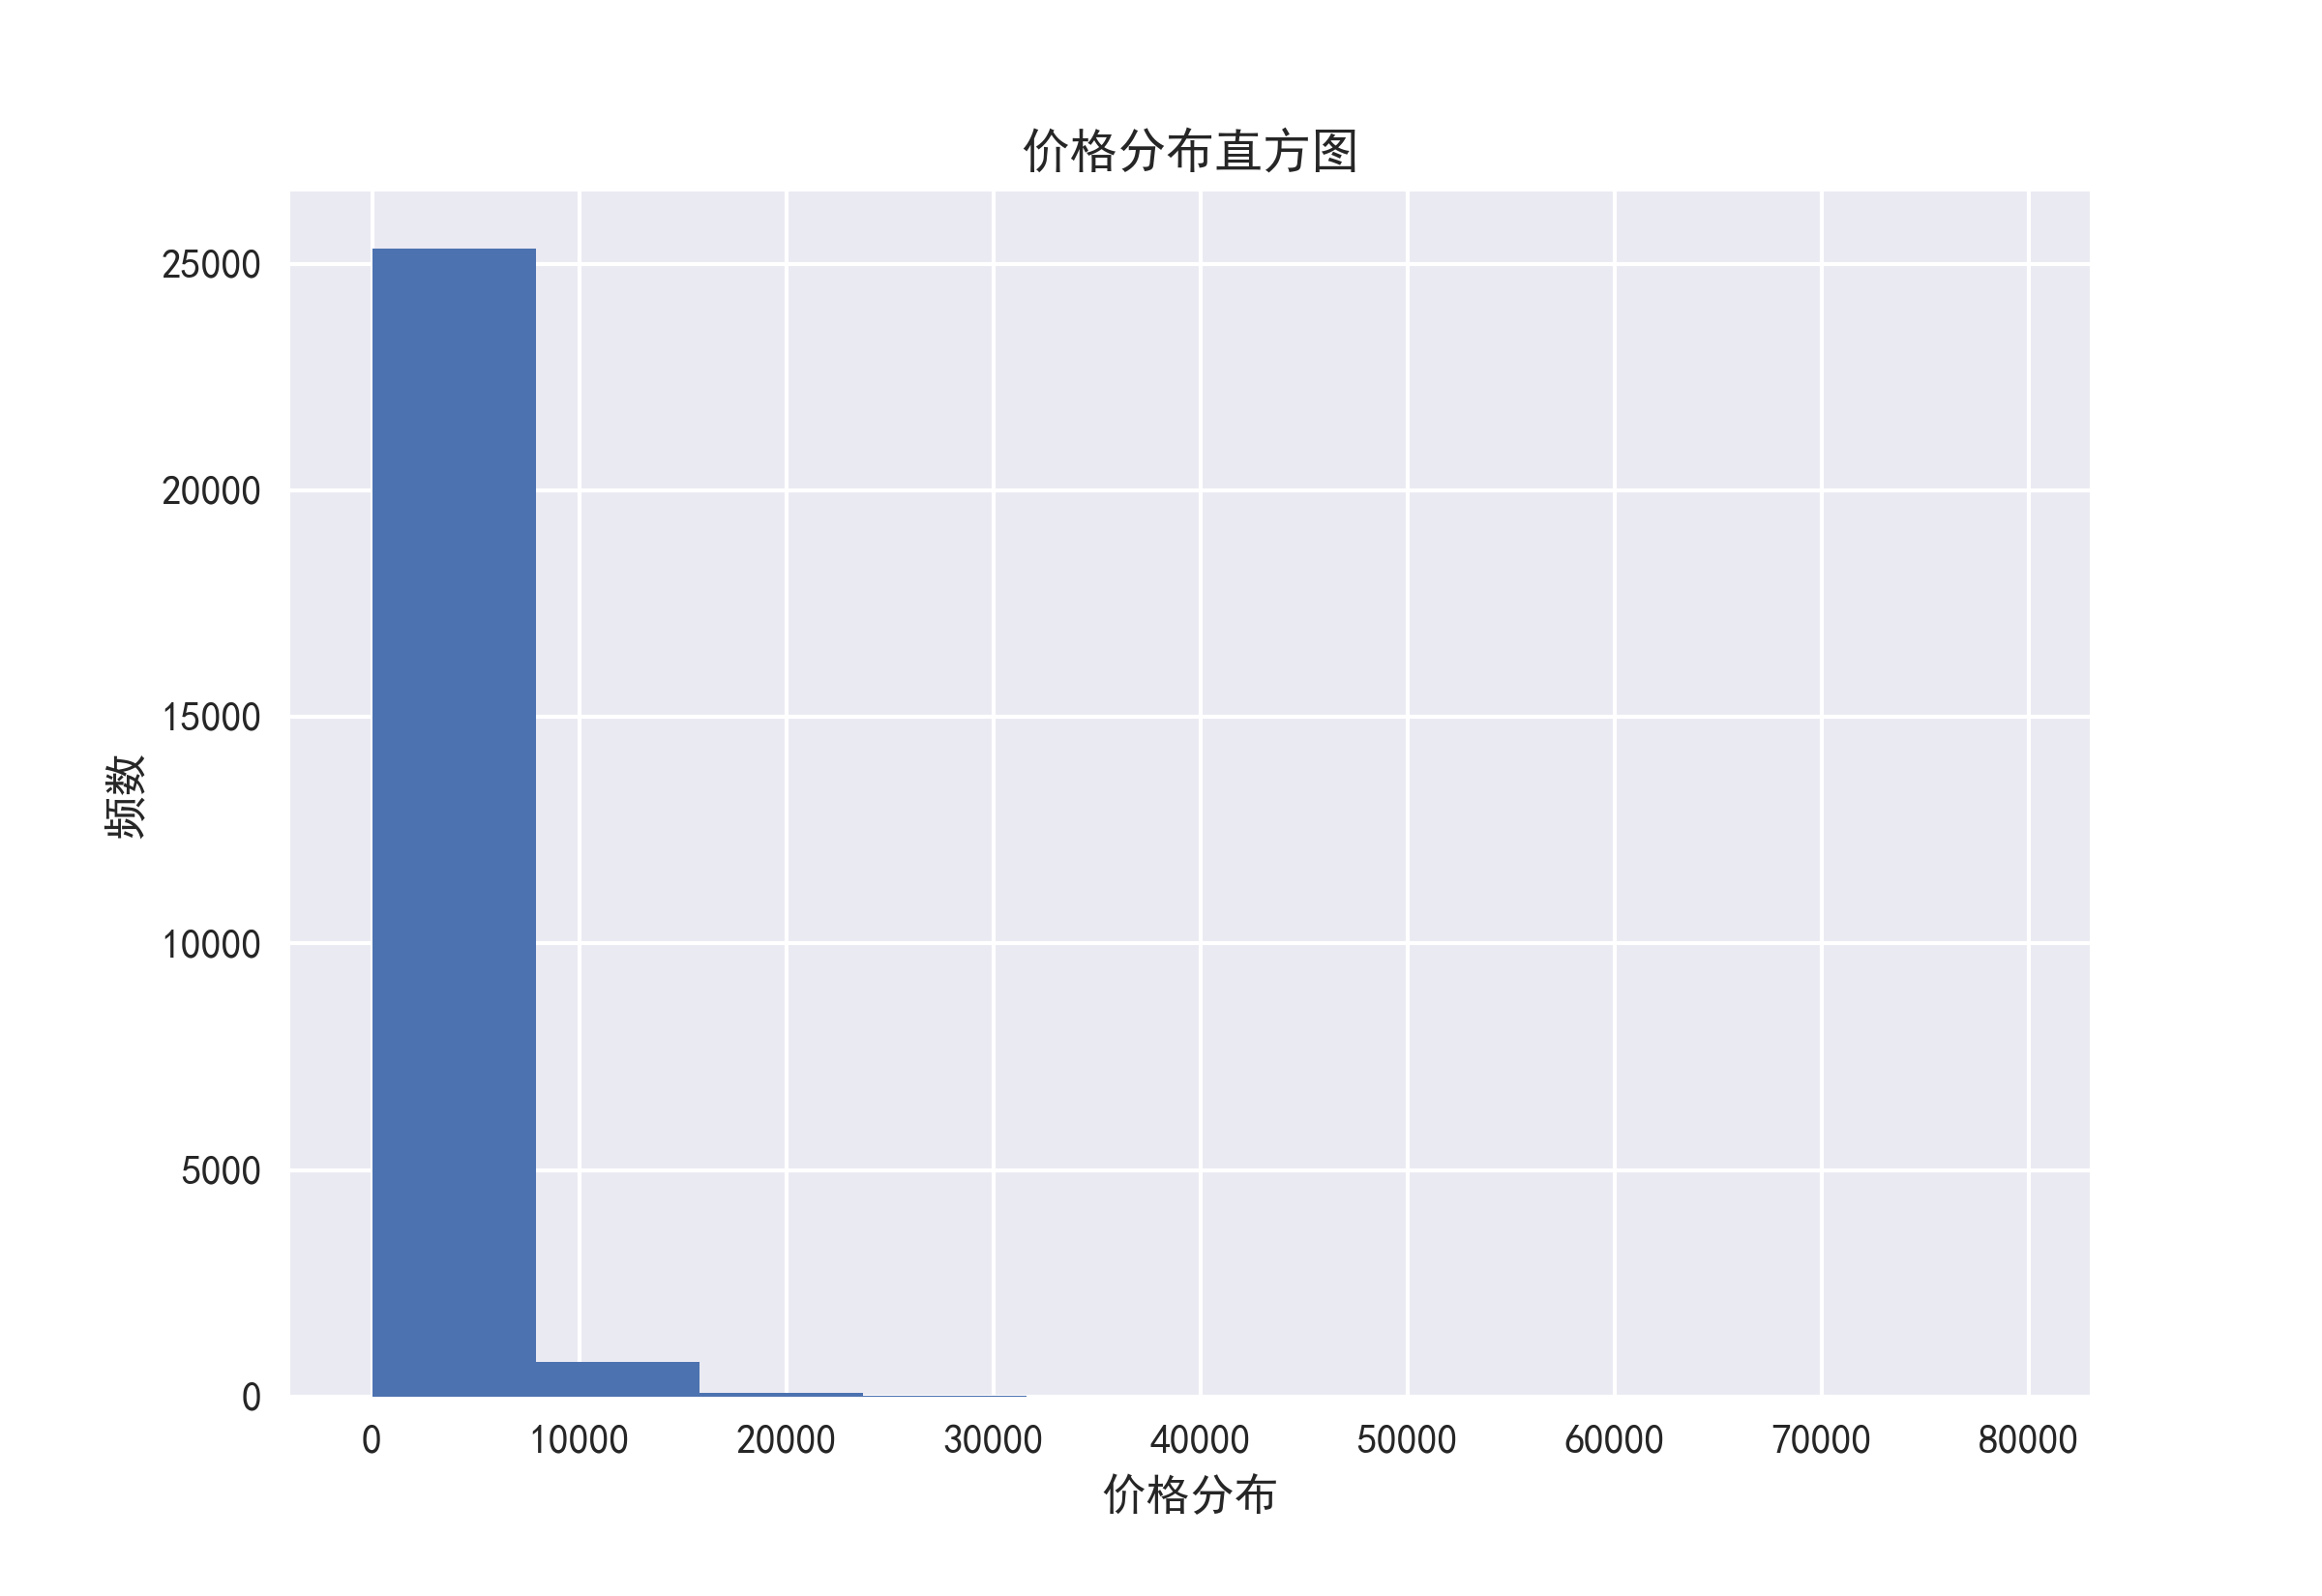
\includegraphics[width=0.45\linewidth]{价格分布直方图}}
	\subfigure[对数价格分布直方图]{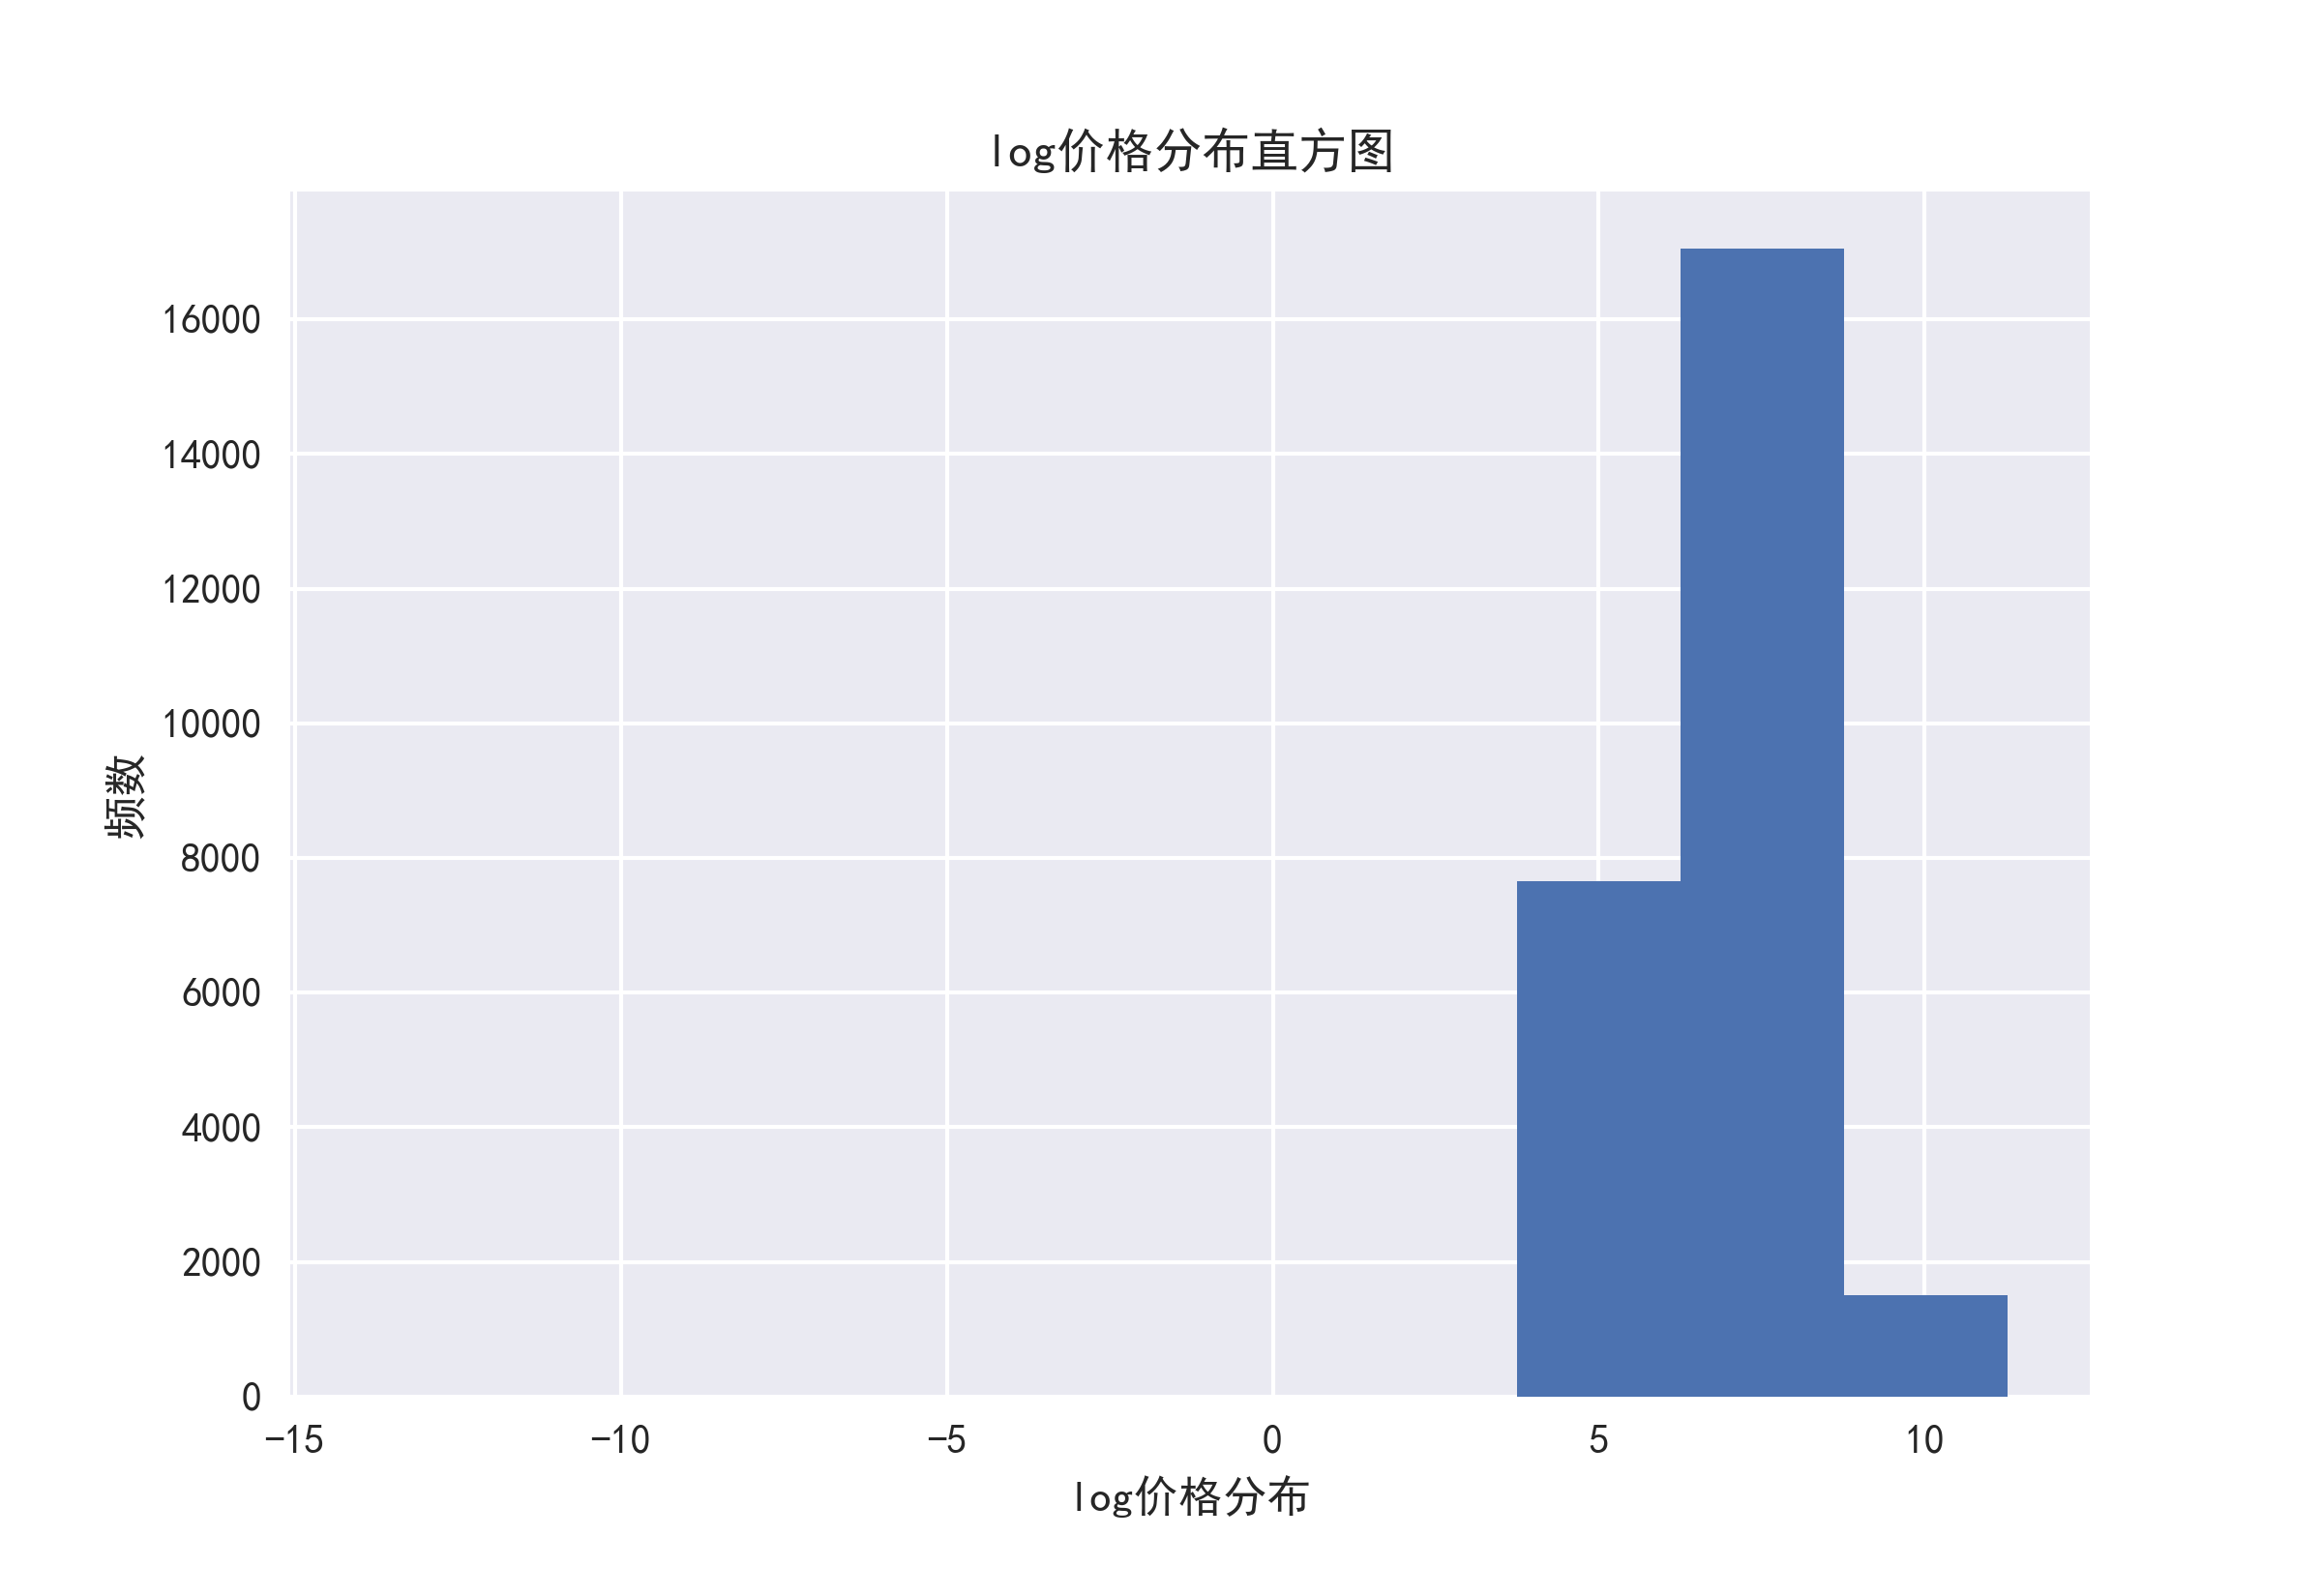
\includegraphics[width=0.45\linewidth]{log价格分布直方图}}
	\caption{价格分布。图中分别展现了对数变换前和变换后的价格分布直方图,其中左图展示出对数变换前,价格呈现明显的偏态分布;对数变换后,价格呈现正态分布。}
	\label{fig:价格分布}
\end{figure*}
\subsection{预订率探索性分析}
\par 房客预订率是机器学习的因变量,通过计算得到。在原始数据的calender表中,每个房源有365天的日历,每个日历上写明了当天价格以及是否可预订。其中可以预定代表着当天没有房客,且房东允许房源被预定;不可预订代表当天有房客已经预定或房东当天不愿意开放房源。在此简单假设房源不可预订意味着该房源当天已经被预定。将统一房源全年中不同的价格进行分组,计算相应组中平均预订率,如公式\ref{公式:平均预订率},其中$y_i$即为分组$i$的平均预订率。
\begin{align}\label{公式:平均预订率}
	\begin{split}
		y_i=\frac{\sum_{j}^{N_i}\mathbf{I_{available}}(j)}{\sum_{j}^{N_i}j}\\
	\end{split}
\end{align}

\par 另外在探索过程中发现了一种异常房源(如图\ref{fig:异常房源}),他们全年都显示为不可预定,这种房源并不是因为房客已经预定而不可定,而是因为房东其实并不想在这个平台上完成预定操作(避免被爱彼迎平台收取抽成),只是在这个平台上展示信息,可以认为这种房源对回归分析是有害的,因此删去这种房源。
\begin{figure*}[tbph]
	\centering
	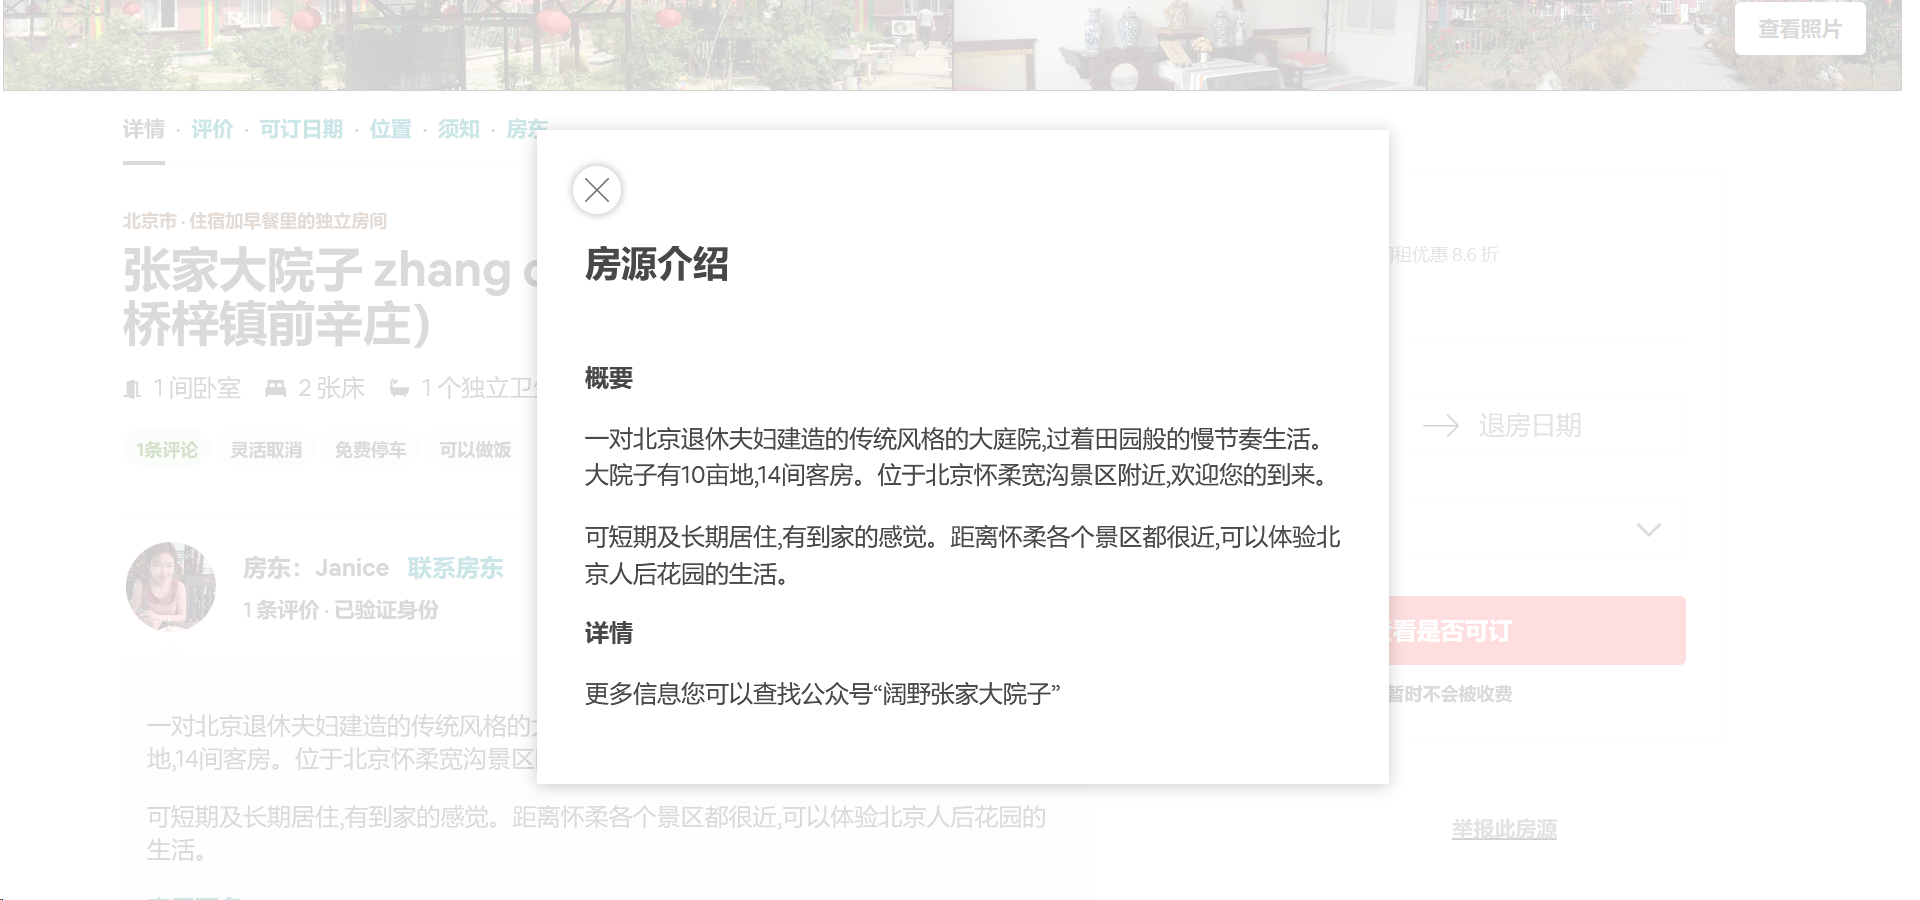
\includegraphics[width=0.8\linewidth]{figures/异常房源}
	\caption[异常房源]{图中展示了一个异常房源的数据,可以看到其他信息基本都是正常的,但在房东介绍可以看到订阅房源只能通过其单独运营的微信公众号完成。}
	\label{fig:异常房源}
\end{figure*}
\subsection{地理数据探索性分析}
其他变量中最重要的是能够反映不同房源地理位置的数据。图\ref{图:房价数据}已经直观的展示了不同地区的房价等分布,图\ref{fig:不同地区民宿个数} 中定量展示了不同的行政区划其房源数量,其中地区6房源占比达到了一半左右,可见不同的行政区其房源数量之间有着巨大的差异,可能和不同地区的经济发展水平、旅游业繁荣程度有密切关系。
\begin{figure}[H]
	\centering
	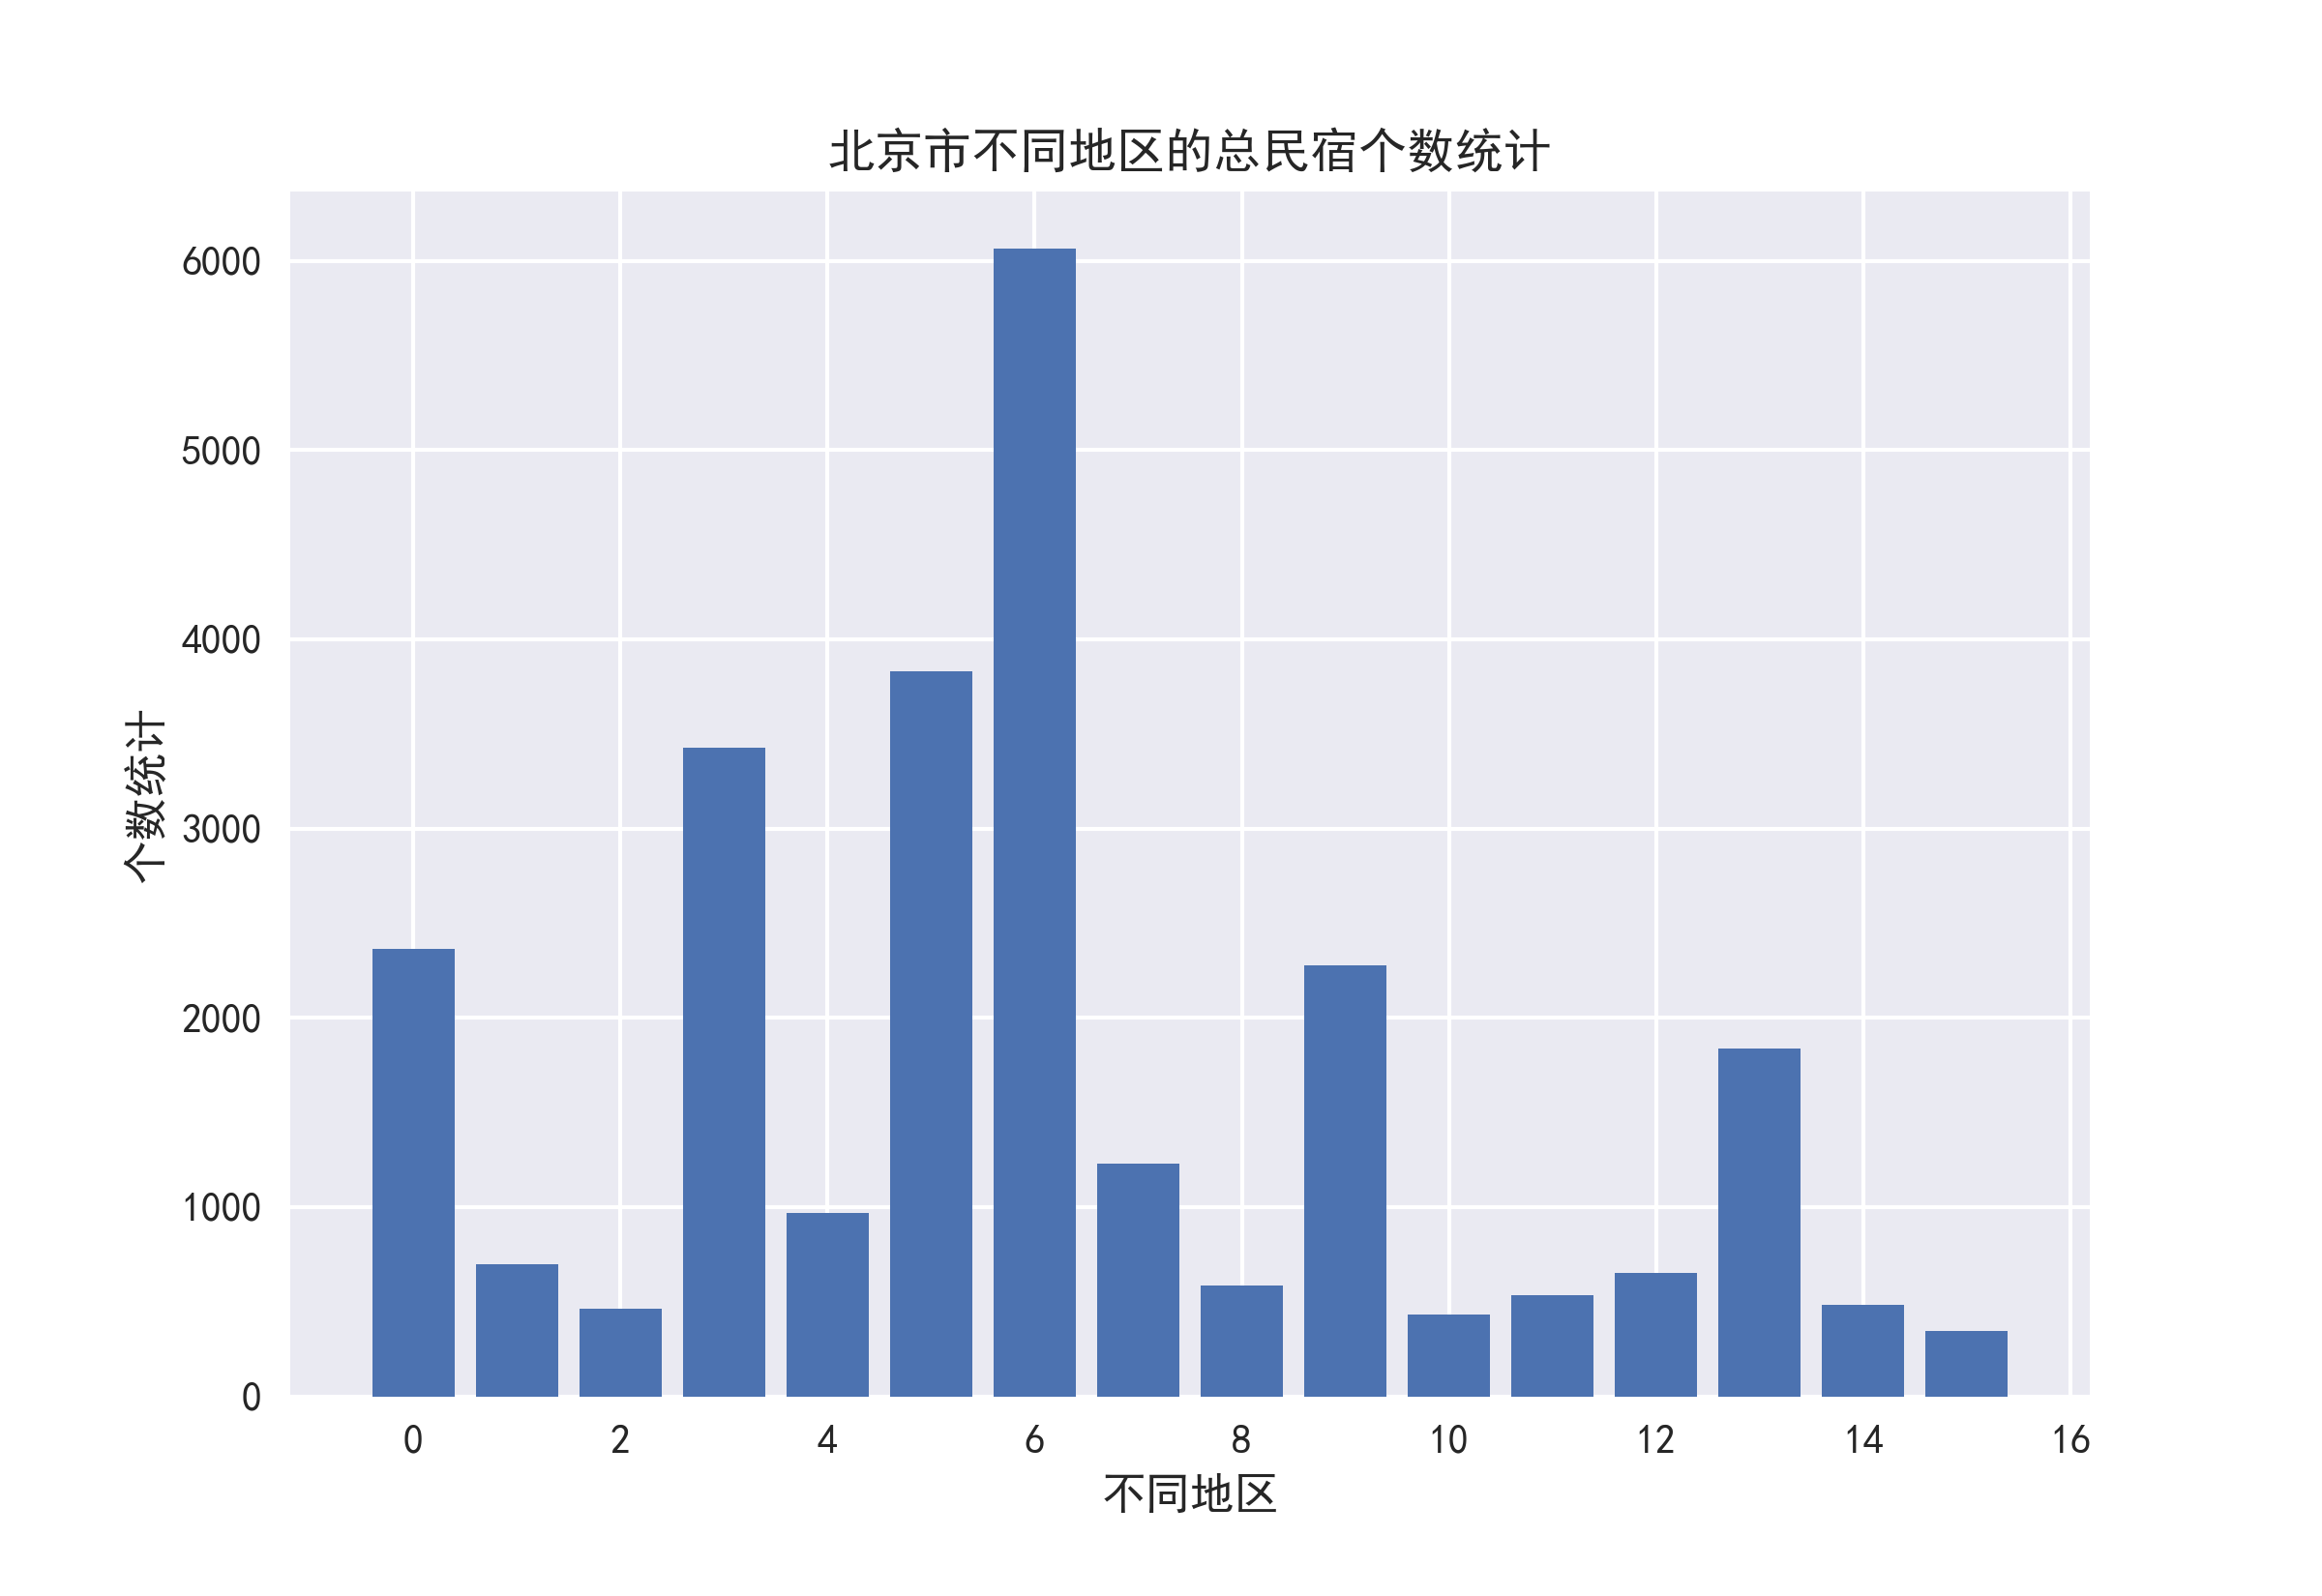
\includegraphics[width=0.7\linewidth]{不同地区民俗个数}
	\caption{不同地区民宿个数统计}
	\label{fig:不同地区民宿个数}
\end{figure}
\subsection{数据相关性探索分析}
\begin{figure}
	\centering
	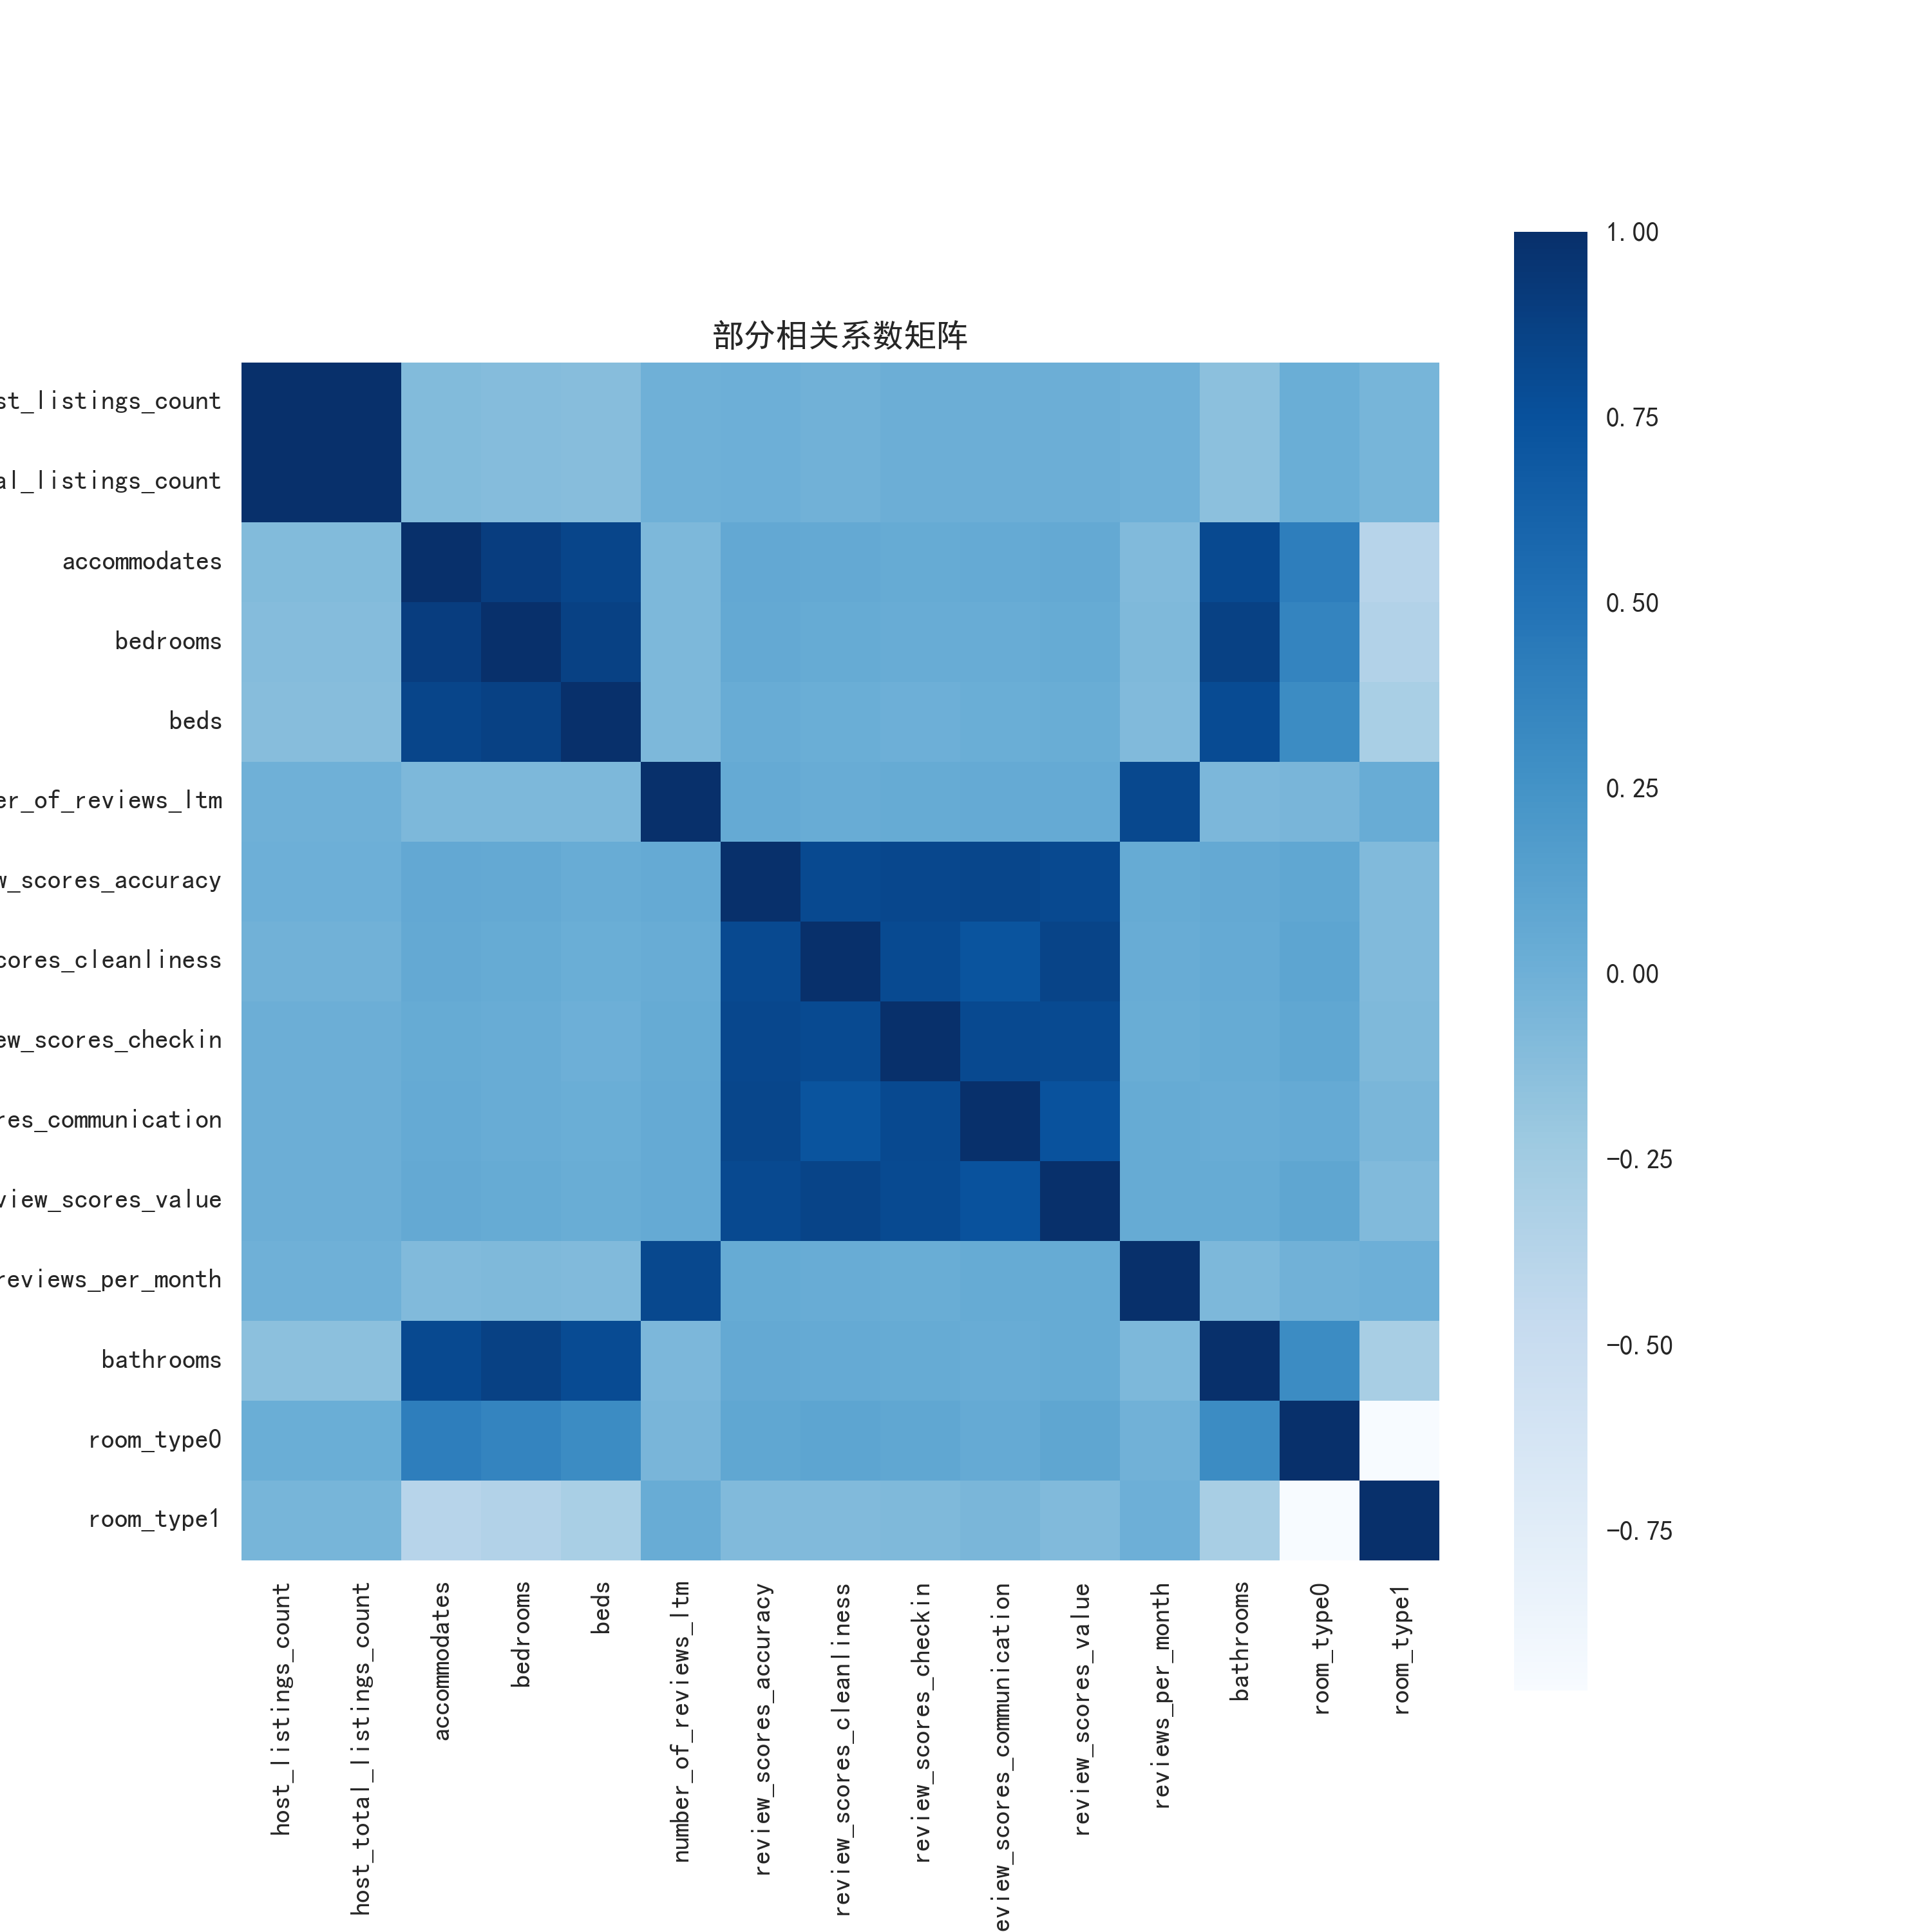
\includegraphics[width=0.8\linewidth]{相关系数矩阵}
	\caption{相关系数矩阵。展示了相关性大于0.8的变量,已经在最新的变量中被删除。}
	\label{fig:相关系数矩阵}
\end{figure}
如图\ref{fig:相关系数矩阵}相关系数矩阵展示了变量间的相关关系,从图中可以看出变量之间大部分呈现浅蓝色,也就是没有很强的相关关系,但是小部分数据之间相关性较强,如“总评分”和“入住时的评分”,将这些小部分相关系数较强的变量删除,有助于在之后的模型中获得令人信服的解释性,因此选择相关性较强的特征进行了删除操作。
\par 图\ref{fig:散点图矩阵}展现了房源价格、预订率、卫生间个数以及是否是地区6(图\ref{fig:不同地区民宿个数})之间的关系。从图中可以看出,价格和预订率之间没有显著的关系,价格和卫生间个数之间有较为明显的正相关关系,但因为这分别衡量了用户的付出和所接收到的服务,没有必要去掉卫生间个数这个变量。而从地理的角度来看,是否是区域6和价格之间有着较为密切的联系,区域6的房源普遍价格偏高,而是否是区域6和预订率、卫生间个数没有很强的正相关关系。而从卫生间个数来看,卫生间个数多少和预订率之间有着并不十分明显的正相关关系。
\begin{figure*}[!htbp]
	\centering
	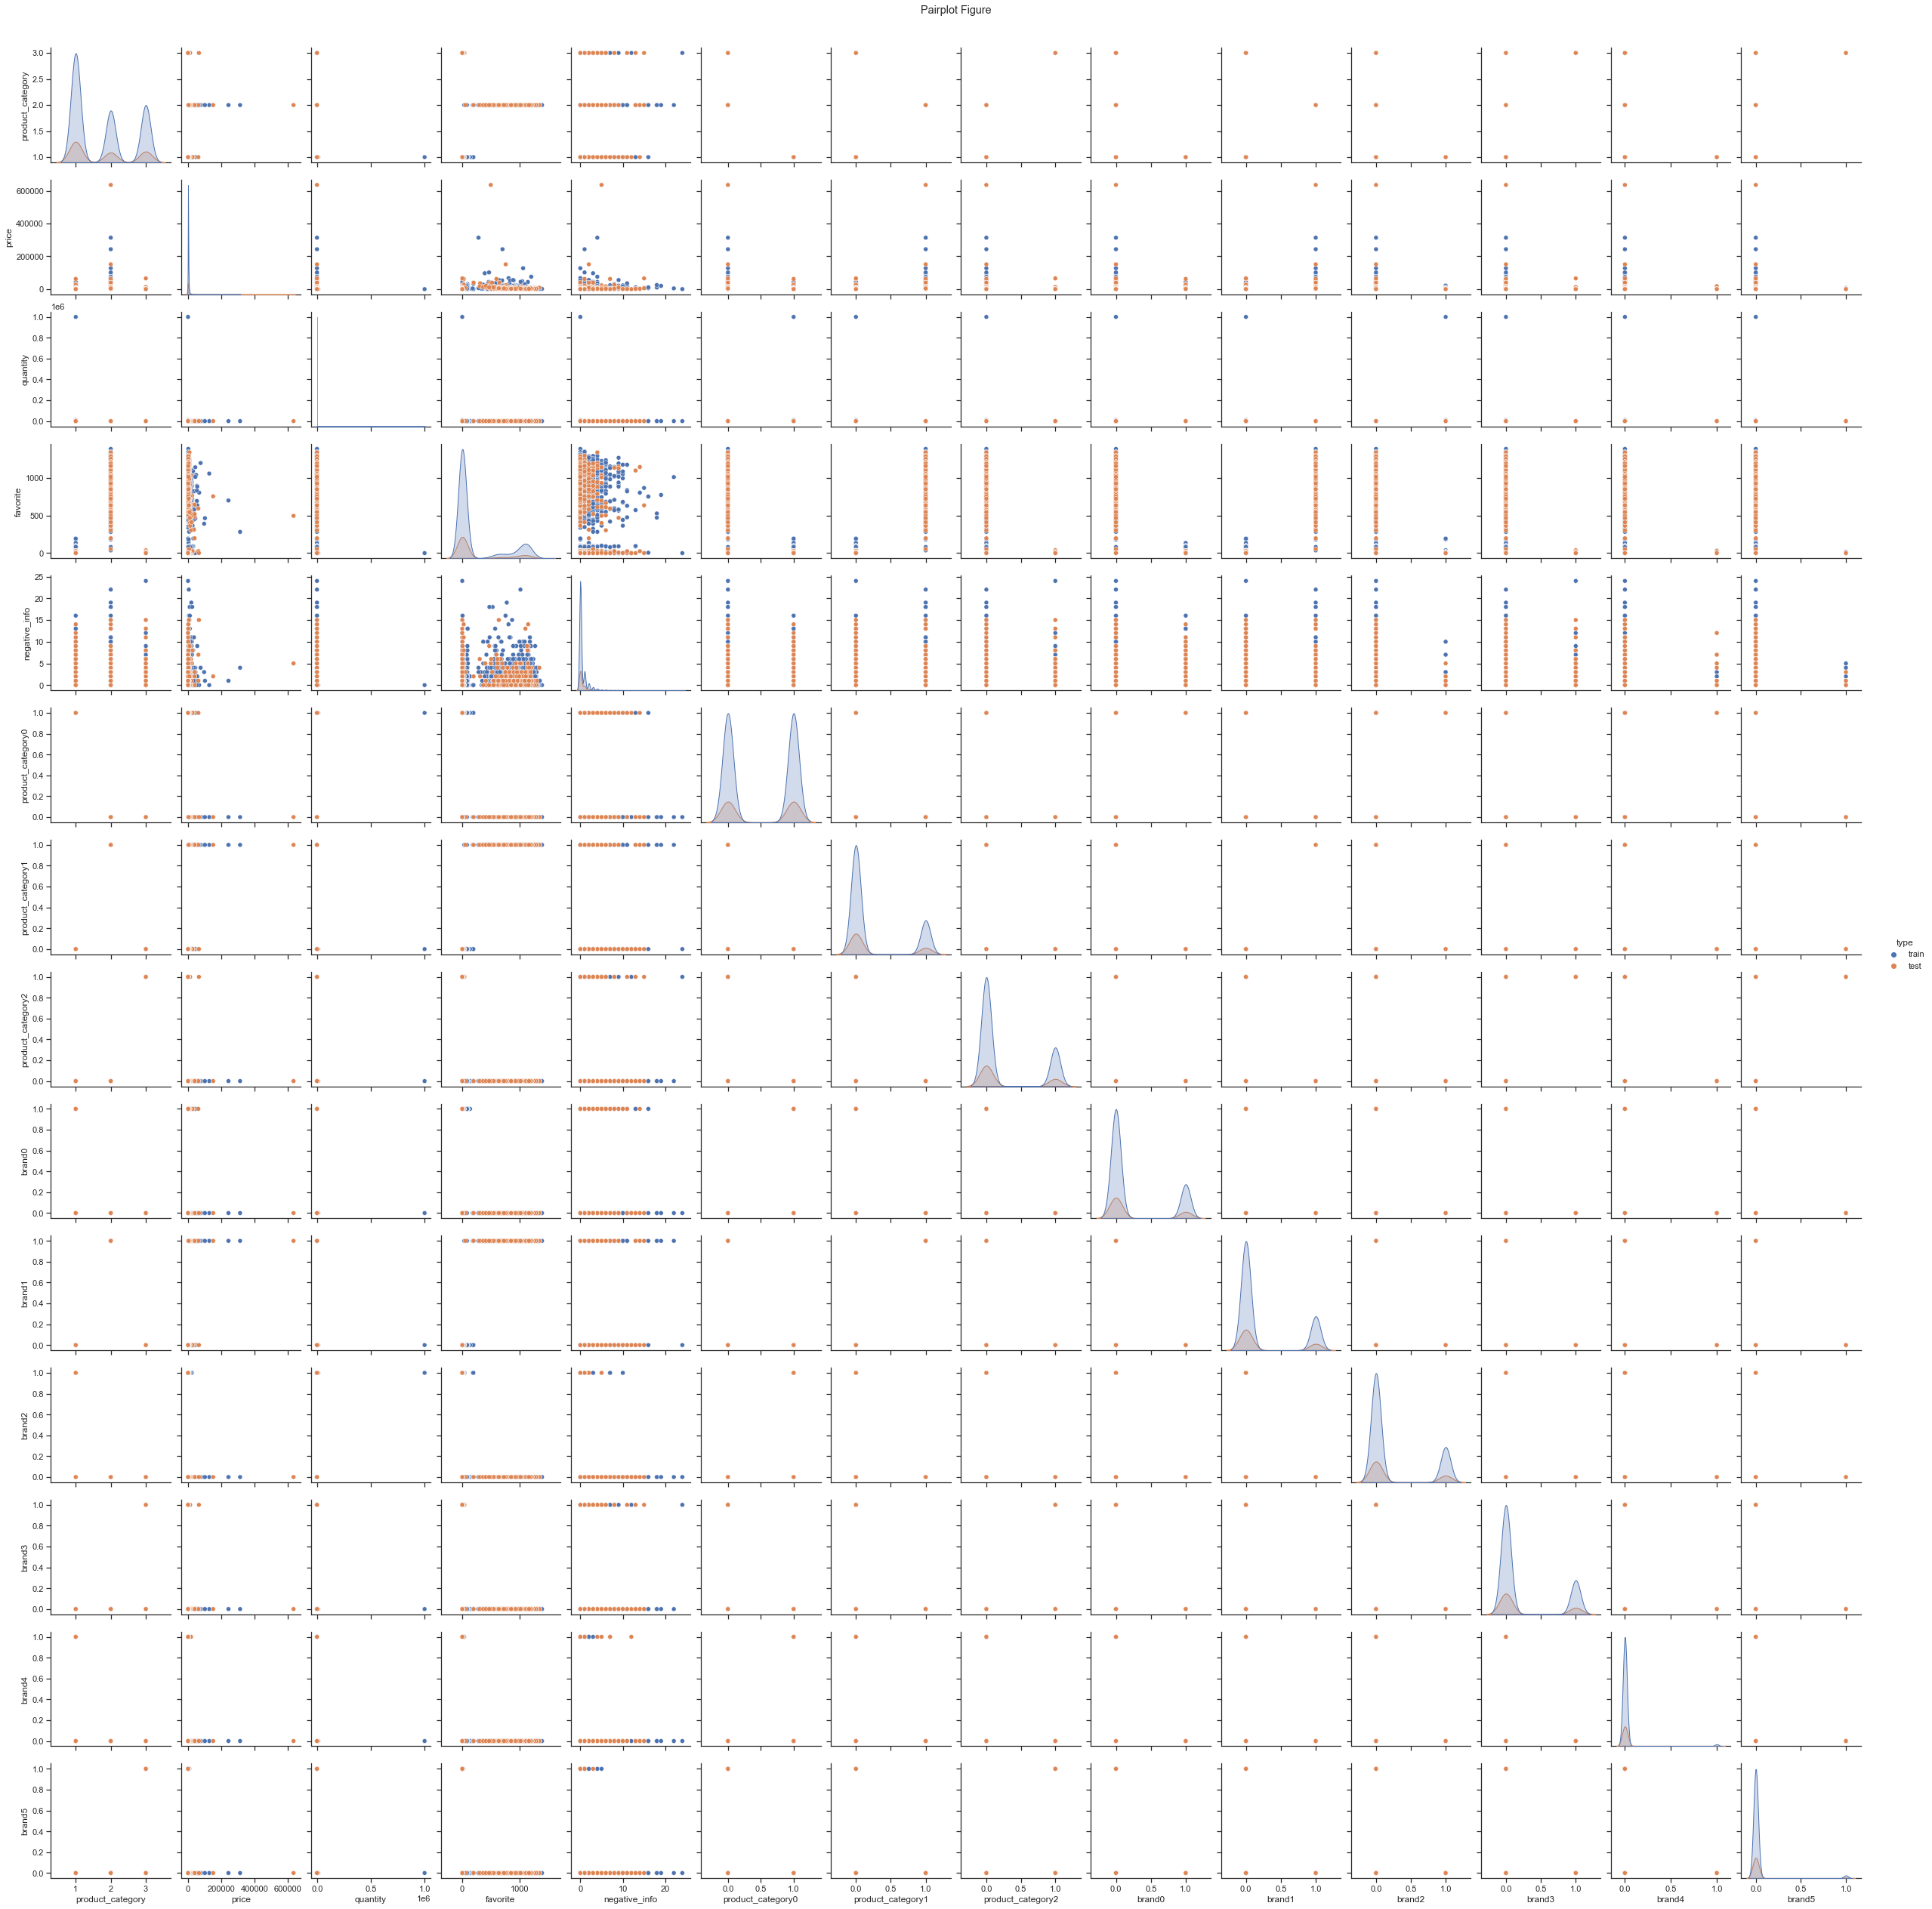
\includegraphics[width=0.9\linewidth]{散点图矩阵}
	\caption{数据相关性探索性分析。取1000个样本绘制,其中不同的颜色代表房源是否是北京的地区6,蓝色代表不位于地区6,黄色代表位于地区6}
	\label{fig:散点图矩阵}
\end{figure*}
\par 综上,不同变量之间的确有关系,但相关关系并不明显,不能使用简单的线性回归方法进行需求预测。

% *** RESULTS ***
\section{方法}
\par 使用弹性网络(ElasticNet),支持向量回归(SVR),LightGBM和多层感知机(MLP)进行模型回归。其中弹性网络回归、支持向量回归使用Scikit-learn\cite{sklearn}实现,LightGBM使用微软的LightGBM包实现\cite{lightGBM},多层感知机使用pytorch\cite{pytorch}实现。
\par 模型参数的选择统一使用hypreopt进行50参数调优完成\cite{hyperopt2022Jan}。每次调优使用五折交叉验证,参数调优的指标选择$R^2$。
\subsection{弹性网络}
弹性网络(公式\ref{公式:elasitcnet},其中$w$为要回归的系数)是一种防止过拟合的改进的线性回归方法。从统计的角度理解,可以认为回归误差在一定程度上满足拉普拉斯分布和高斯分布的混合分布,利用罚函数可以强制要求最后回归的结果在一定程度上满足两种分布,从而获得更小的泛化误差。但是因为这只是线性回归增加了罚函数,不能期望在复杂的拟合问题中有着优秀的表现,这里选择弹性网络只是作为基函数,作为评价其他模型的下限。
\begin{align}\label{公式:elasitcnet}
\frac{1}{2\times N} \times ||y-Xw||_2^2+\alpha \times l1_{ration}\times ||w||_1 +0.5 \times \alpha \times (1-l1_{ratio})\times ||w||_2^2 
\end{align}
\subsection{支持向量回归}
支持向量机模型自提出之后就有在诸多问题中有着优秀的表现,并获得了广泛的应用,支持向量回归主要用来优化问题\ref{公式:SVR}。
\begin{align}
	\begin{split}\label{公式:SVR}
		\min_{w,b,\xi,\xi^*} \frac{1}{2}||w||^2+C\sum_{i=1}^{m}\xi_i^+C\sum_{i=1}^{m}\xi_i^*\\
		s.t. \quad w^T\Phi(x^i)+b-y^i&\leq \epsilon+\xi_i\\
		y^i-w^T\Phi(x^i)-b &\leq \epsilon +\xi_i^*\\
		\xi_i,\xi_i^* \geq 0,i=1,...,m 
	\end{split}
\end{align}
\subsection{LightGBM}
集成学习算法是另外一种典型的算法,其中应用最广泛的是GBDT算法,据统计Kaggle比赛中一半以上的冠军算法是基于GBDT实现的。微软开发了LightGBM\cite{lightGBM}算法框架用以实现GBDT。LightGBM算法还有一个优点是可以给出特征的重要程度,本文以决策树为基学习器,尝试利用LightGBM进行预测。
\subsection{多层感知机}
多层感知机模拟人类的神经网络进行学习,通过搭建互相连接的多层神经元,在理论上可以模拟任意复杂的函数,在图像分类、文本挖掘领域有着重要应用。本文利用pytorch搭建两个隐层的神经网络,观察他的效果。
\subsection{调优之后选择的参数汇总}
利用hyperopt进行参数调优之后,选择了如表\ref{tab:参数汇总}所示的参数。
\begin{table}[H]
	\centering 
	\begin{tabular}{|c|cc|}
		\hline 
		模型名称 & 参数名称 & 参数值 \\\hline 
		\multirow{2}{*}{弹性网络} & $\alpha$ & 0.12\\  
		 & $l1_{ratio}$ & 0.14 \\\hline 
		 \multirow{2}{*}{SVR} & $C$ & 0.33 \\
		  & $\gamma$ & 0.09\\\hline
		  \multirow{4}{*}{LightGBM}
		  & $learning\_rate$ & 0.04\\
		  & $max\_depth$ & 0\\
		  & $n\_estimators$ & 140\\
		  & $num\_leaves$ & 80\\\hline 
		  \multirow{5}{*}{多层感知机} & $batch\_size$ & 1000\\
		  
		  & $epoch$ & 60\\
		  & 隐层1神经元个数 & 94\\
		  & 隐层2神经元个数 & 72\\ 
		  & $learning\_rate$ & 0.0004\\\hline  
	\end{tabular}
\caption{参数汇总}
\label{tab:参数汇总}
\end{table}

\section{结果}
选用MAE,MSE,R2作为回归分析的主要指标进行评价。不同模型的结果如表\ref{tab:模型评价},可见弹性网络的性能明显低于其他回归方法的性能,在此印证了机器学习回归方法的必要性。
\begin{table}[H]
	\centering
	\begin{tabular}{|c|ccc|ccc|}
		\hline
		\multirow{2}{*}{模型名称} &  \multicolumn{3}{c|}{训练集}       &  \multicolumn{3}{c|}{测试集}  \\
		\cline{2-7}
			&      MAE  &  MSE     &    $R^2$   &   MAE     &   MSE    &  $R^2$\\ 
		\hline 
		弹性网络 & 0.450 & 0.257 & 0.029 & 0.349 & 0.157& 0.047 \\	  \hline 
		支持向量回归 & 0.293 & 0.181 & 0.306 & 0.223&0.132 & 0.230  \\	 \hline 
		LightGBM & 0.275 & 0.1160 & 0.335 & 0.2999 & 0.130 & 0.1662 \\	 \hline 
		多层感知机 & 0.301 & 0.1179 & 0.2340 & 0.234 & 0.107 & 0.245\\	 \hline 
	\end{tabular}
\caption{模型评价}
\label{tab:模型评价}
\end{table}
\par 如图\ref{fig:预测-真实预订率}展示了用LightGBM预测的数据和真实的数据的展示,总体来说大部分结果都在真实值左右,没有很严重的偏差。
\begin{figure}[H]
	\centering
	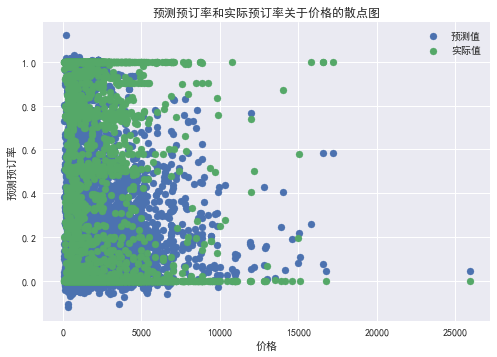
\includegraphics[width=0.8\linewidth]{预测-实际-预订率}
	\caption{预测和实际的预订率。图中绿色标签为真实情况,蓝色标签为LightGBM模型计算的结果,横轴为价格,纵轴为预订率。}
	\label{fig:预测-真实预订率}
\end{figure}
\par 如表\ref{tab:模型评价},在训练集和测试集中,模型表现最好的均是lightGBM,为了探究什么变量更为重要,获取了lightGBM给出的特征重要性评价,如表\ref{tab:特征重要性},可以看出在各个特征中价格确实是影响预订率最重要的特征,这和经济学的的假设相符;在其他特征中,房源建立时间、地理状况和平均评论情感是所有特征中更为重要的因素,展现出房客更加重视这些,这和前人的关于OTA酒店等关键因素的研究结果较为一致。因此北京市的房东更应该关注这些因素,加强 房源品牌的建设,建立良好的口碑,坚持长期经营的战略等。
\begin{table}[!htpb]
	\centering
	\begin{tabular}{c|c}
		\hline 
		特征名称  & 重要性\\\hline
		价格(取对数) & 3874 \\
		房源成立时间 & 1599 \\
		纬度 & 1536 \\
		经度 & 1496\\
		平均评论情感 & 992 \\\hline 
	\end{tabular}
\caption{LightGBM特征重要性排序}
\label{tab:特征重要性}
\end{table}
\section{典型房东分析}
为了将经济学理论和机器学习模型相结合,给出对于房东更有价值的建议,在本章中选取典型房东,研究随着他们的定价发生变化,在预订率方面会怎样变化,从而怎样定价才能提高收入。
\begin{figure*}[!htbp]
	\centering
	\subfigure[房源1]{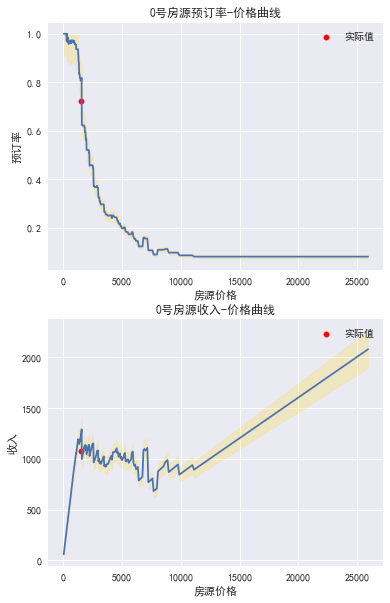
\includegraphics[width=0.24\linewidth]{好房源1}}
	\subfigure[房源2]{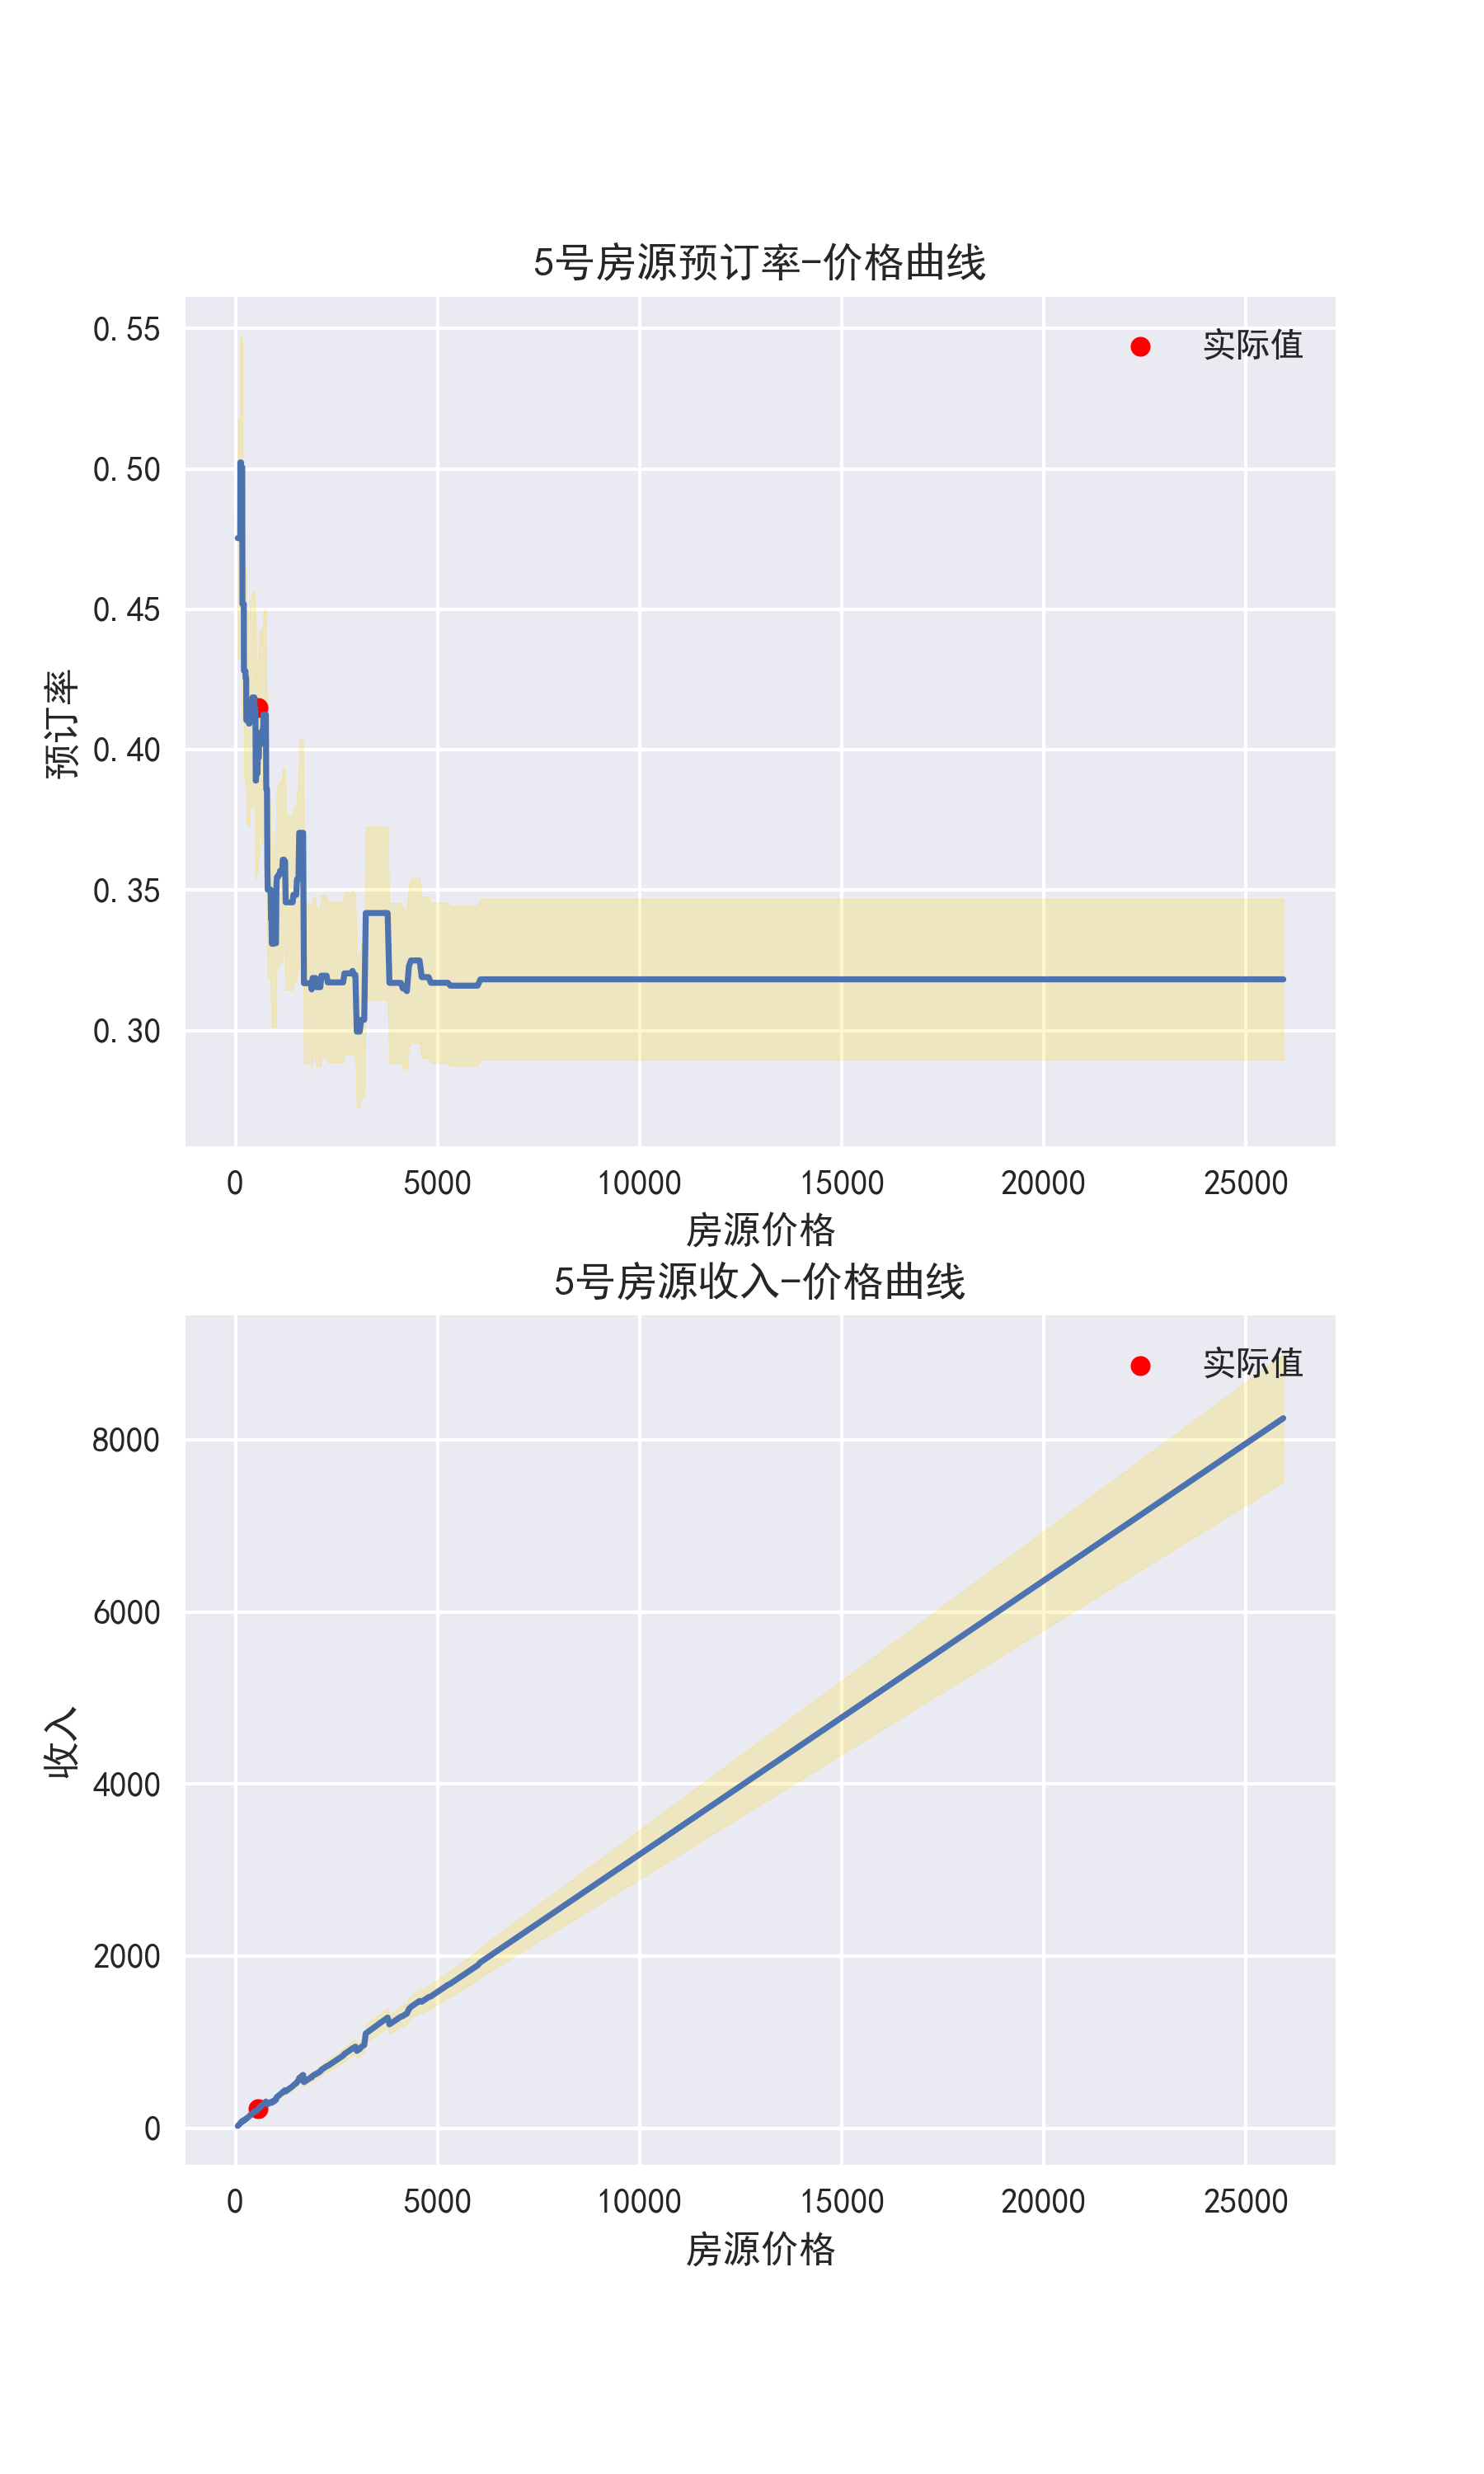
\includegraphics[width=0.24\linewidth]{普通房源1}}
	\subfigure[房源3]{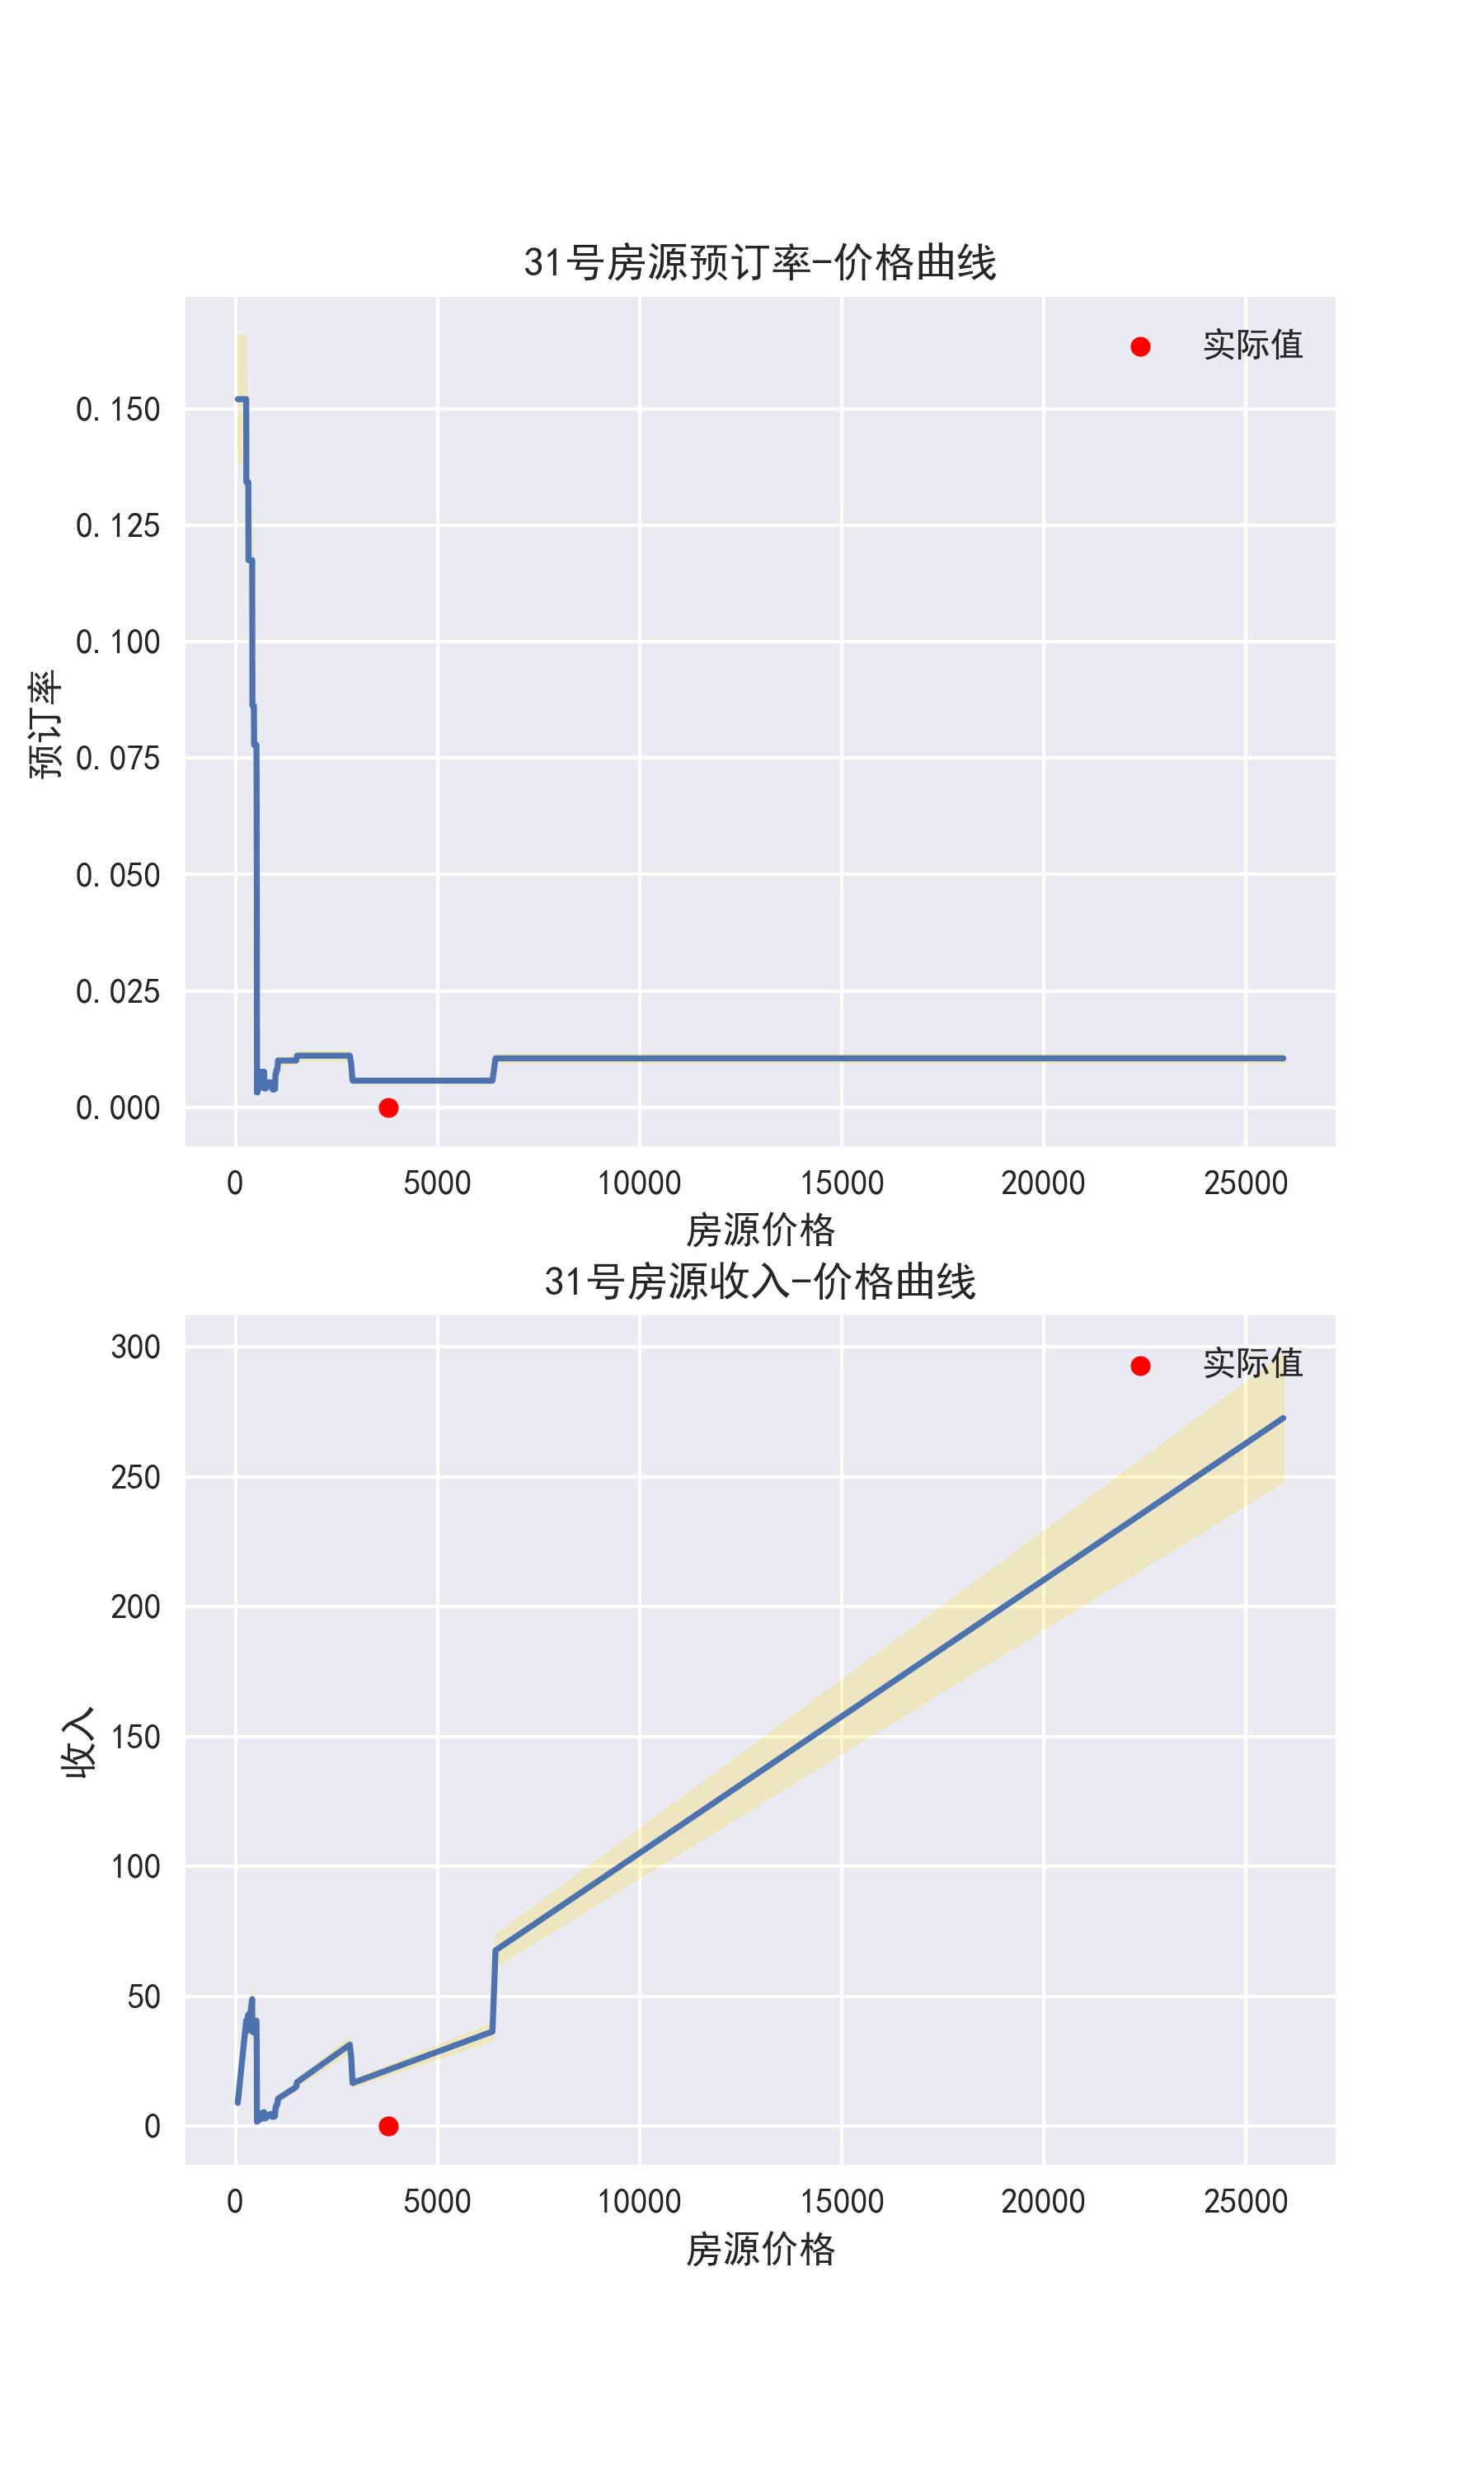
\includegraphics[width=0.24\linewidth]{坏房源1}}
	\subfigure[房源4]{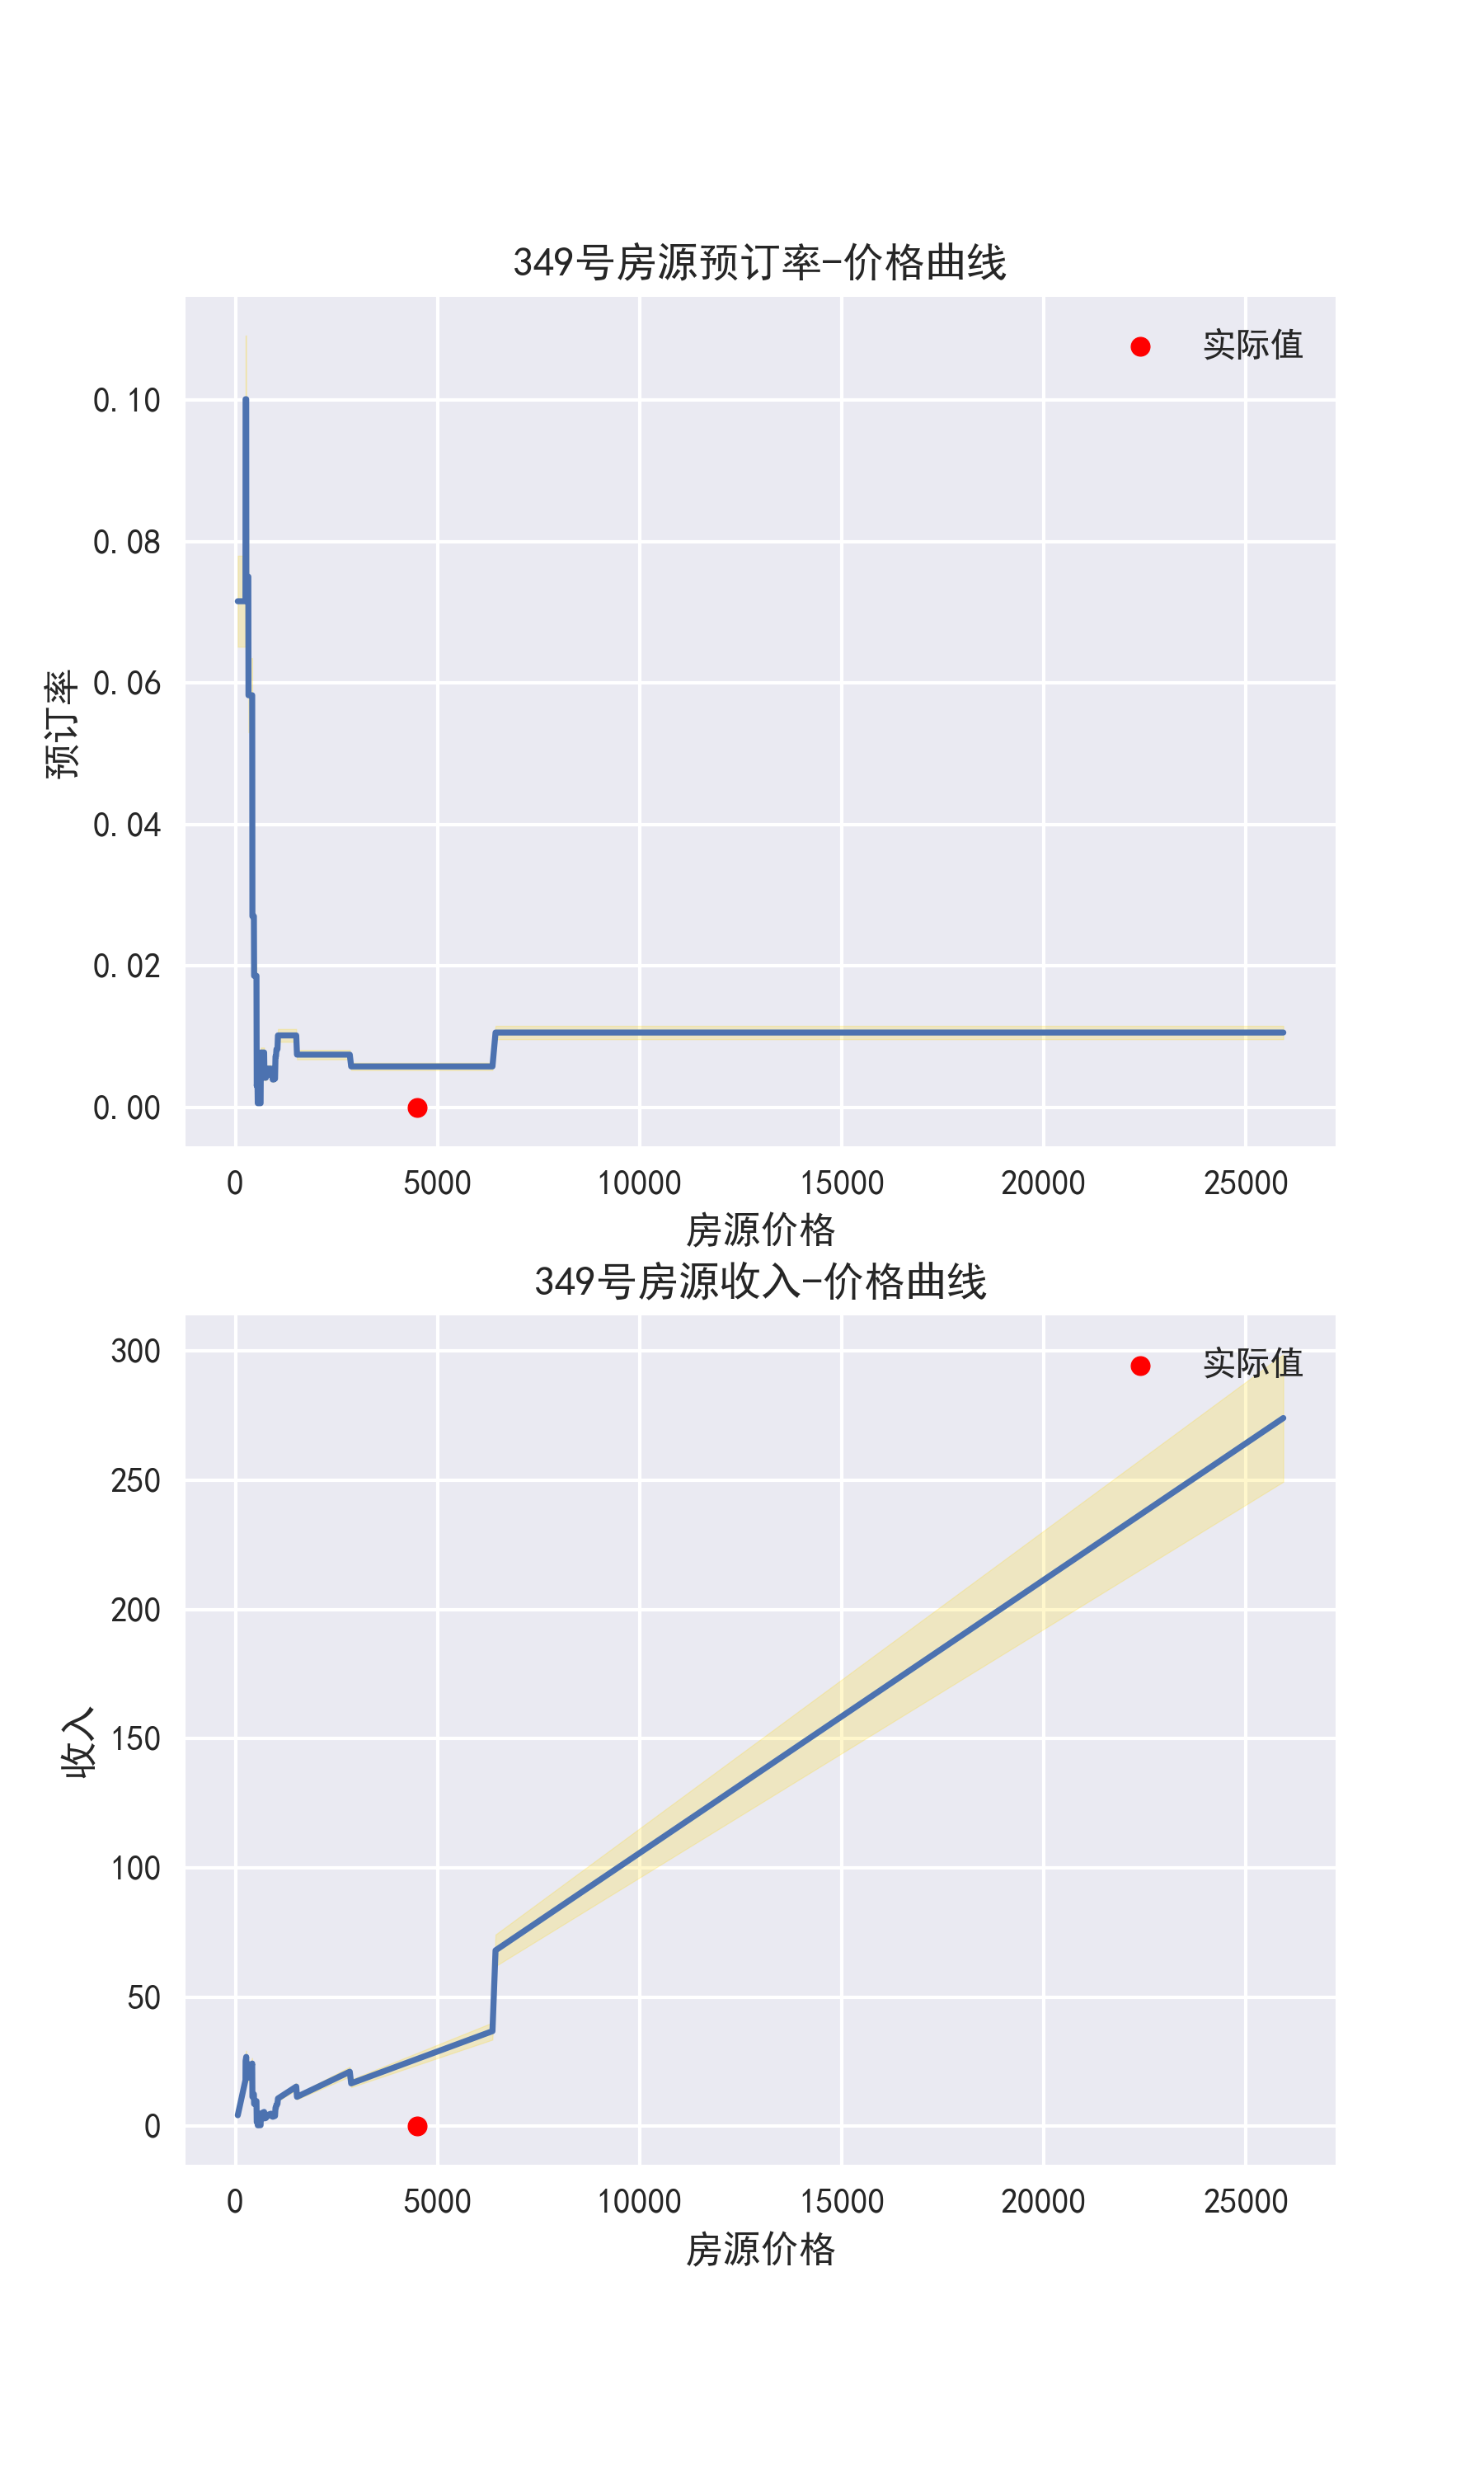
\includegraphics[width=0.24\linewidth]{坏房源2}}
	\caption{4个不同典型房源。其中房源1是经营状况较为理想的房源、房源2是经营状况较为普通的房源、房源3和房源4经营状况较为不理想。每个房源上图是预测的房源价格与预订率的关系,总体都呈现下降趋势;下图展示的是房源价格和预测收入的关系。图中黄色区域是预测结果的一个标准差的范围,代表置信区间。}
	\label{fig:典型房源}
\end{figure*}
\par 首先定义房东的运营情况好坏,房东运营指标$f$如公式\ref{eq:运营}。该指标考虑到之前分析得到的不同地理位置会很大程度上影响房东的收入,因此按照北京市不同的行政区划分区进行计算,每个区计算房源平均价格和房源平均预订率,定义平均收入为平均价格$\times$ 平均预订率,房东相应的价格$\times$ 预订率定义为房东的预期收入,用房东的预期收入减去该地区的平均收入即为房东的运营指标$f$,显然,该指标取值范围为$f \in R$,且$f$越大,房东运营状况越好,$f$最低的基本可以说明运营是有问题的。
\begin{align}\label{eq:运营}
	\begin{split}
		f(x)=AP(x)&\times BR(x) -\bar{AP_{Ng}}\times \bar{BR_{Ng}}\\ \bar{AP_{Ng}}&=\frac{\sum_{i=1}^{N_g}AP_{i}}{\sum_{i=1}^{N_g}i}\\
		\bar{BR_{Ng}}&=\frac{\sum_{i=1}^{N_g}BR_{i}}{\sum_{i=1}^{N_g}i}\\
		for \quad N_g=\left[x\right],AP&=Adjusted\_price,BR=Booking\_Rate
	\end{split}
\end{align}
\par 选取了如图\ref{fig:不同地区民宿个数}中民宿数量最多的五个地区计算每个房东的运营状况,分别选取了其中运营较为良好,运营状况最差、运营状况一般共5个房东。按照价格从该地区最低到该地区最高的顺序生成模拟价格,替换原来该房源的价格特征。根据调参结果,选择LighhtGBM调整好的超参数,把训练集和测试集合并作为数据集进行训练得到模型$M$,利用$M$对这些数据进行预测,得到如图\ref{fig:典型房源}所示预测结果。

\par 首先可以看到普遍来说需求与价格之间呈现负相关关系,而不同的房源具体的需求曲线是不同的,有些房源需求曲线在某些价格水平下反而上升。首先看经营性良好的房源1,从图中可以看到如果房源1价格提升,如厕需求会显著下降,从价格-收入曲线可以看到房源的收入会随着房源价格的上升震荡,考虑到预测的随机性,的确不适合改变价格;房源2的需求也会随着价格的上升而显著下降,但是从收入曲线来看,应该适当提价;房源3和房源5的需求曲线大致相同,在目前的定价水平下都无法获得可观的收益,预测发现降价策略可以大幅提高需求,应该选择降价策略;房源4虽然需求也较低导致收入偏低,但与另外两处房源不同的是,提价策略有可能获得收入:这可能和房源本身定位比较高有关系,这种房源在这种价位的可能反而收受不到目标客户的信任,提升价格的策略反而是奏效的。
\par 综上,从图中可以看出机器学习的结果依然有不准确的地方,比如在多个房源的预测中,当价格偏高到一定程度时,反而使得房源预期收入上升,这和收集到的数据不能完全反应房源本身的质量有关,也是之后的改进方向。
\section{结论}
本研究主要利用机器学习的模型预测北京爱彼迎平台上不同房源的定价的需求,从而尝试为房东提出合理的定价建议来提高收入。
\par 本文首先处理了原始变量,对不同时间范围内的价格进行分组聚合,并对价格进行了对数变换降低其偏度,对用户评论数据进行了情感分析,并对其他变量进行了独热编码、格式转换等。之后分析了价格、地理位置等重要变量的分布和区间信息,以及在若干在出探索阶段认为比较重要的变量之间的相关关系,发现这些变量之间以及这些变量和因变量之间普遍没有很强的相关性,这和传统酒店的定价管理面临的模式是不同的,因此使用更复杂的机器学习模型学习这些数据以辅助决策是有必要的。在前人研究的基础上,选择了弹性网络回归作为用来比较的基础模型,选择支持向量回归、LigthGBM和多层感知机三种目前主流的机器学习模型来比较最终预测的性能。
\par 选择预测性能最好的LightGBM模型,分析特征的重要程度,发现最重要的特征包括对数变换后的价格、地理分布、房源时长以及客户平均评价是影响用户需求最重要的变量,商家应该着重于选择地理位置条件更好的、更热门的地区进行商户开设,商家也应该坚持运营好与顾客之间的关系,坚持以质取胜,做好长期运营,做长品牌的工作。
\par 尝试利用模型寻找典型房东,参考前人的研究,利用聚类的思想评价房东的运营状况,利用LightGBM训练得到的模型预测几位房东在不同的定价策略下可能的需求量,从而计算出相应的收入。结果发现不同的房东应该考虑不同的定价策略,大部分房东可能需要降价提高需求量;而少部分房东,需求量偏低却可能是由于价格过低,应该提高价格,从而有可能提高需求量兵器高收益率。可以看出模型本身具有一定的参考价值。
\par 在此使用的经济学模型有其固有缺陷,即从需求影响价格的角度进行刻画,没有充分考虑供给的问题。但缺陷主要来自于收集的数据主要是从房客的角度进行收集,在刻画需求方面有先天的优势,比如通过用户评价、用户打分等刻画了满意度,通过房屋类型刻画了不同用户的需求;但从供给的角度——即劳动的价值角度,没有办法准确得刻画,比如没有办法准确刻画房源的内部装饰等,房源的准确面积,房东准确的劳动投入等,虽然有相应的替代指标,但这些指标也并不准确,存在大量偏差。正如马克思指出的那样,价格的决定因素是价值,即劳动投入,笔者认为这也是这个模型在预测需求方面产生偏差的根本原因。至于改进,在接下来的研究中应该加大在供给角度的刻画,比如可以进一步分析房源的展示图片从而进一步刻画房东的劳动投入。
\par 另外,从时空范围来看,模型也有着不可避免的缺陷。研究仅限于北京一个地方,而且北京市由于特殊的管制政策,房源数量普遍低于纽约、东京、上海和香港等大都市,导致研究结果并不准确,也没有进一步研究这个模型能否适用其他城市的房源,导致普适性不足。没有区分节假日等特殊时间段,导致很多价格的变动的原因不能被准确捕捉,最后的模型也就容易出现性能不佳的问题。
\par 总体而言,这个模型虽然大大简化了真实世界,但在偏差方面基本可以接受,可以为房东定价提供一定的指导和建议,也为下一步的研究开辟了道路。
\section{代码获取}
关于代码的说明放在了Readme文件中。

\end{multicols}
% *** REFERENCES ***
\newpage
\bibliography{bibliography}
\bibliographystyle{naturemag}

\end{document}
